% This is the Reed College LaTeX thesis template. Most of the work 
% for the document class was done by Sam Noble (SN), as well as this
% template. Later comments etc. by Ben Salzberg (BTS). Additional
% restructuring and APA support by Jess Youngberg (JY).
% Your comments and suggestions are more than welcome; please email
% them to cus@reed.edu
%
% See http://web.reed.edu/cis/help/latex.html for help. There are a 
% great bunch of help pages there, with notes on
% getting started, bibtex, etc. Go there and read it if you're not
% already familiar with LaTeX.
%
% Any line that starts with a percent symbol is a comment. 
% They won't show up in the document, and are useful for notes 
% to yourself and explaining commands. 
% Commenting also removes a line from the document; 
% very handy for troubleshooting problems. -BTS

% As far as I know, this follows the requirements laid out in 
% the 2002-2003 Senior Handbook. Ask a librarian to check the 
% document before binding. -SN

%%
%% Preamble
%%
% \documentclass{<something>} must begin each LaTeX document
\documentclass[12pt,twoside]{reedthesis}
% Packages are extensions to the basic LaTeX functions. Whatever you
% want to typeset, there is probably a package out there for it.
% Chemistry (chemtex), screenplays, you name it.
% Check out CTAN to see: http://www.ctan.org/
%%
\usepackage{graphicx,latexsym} 
\usepackage{amssymb,amsthm,amsmath}
\usepackage{longtable,booktabs,setspace} 
\usepackage{chemarr} %% Useful for one reaction arrow, useless if you're not a chem major
\usepackage[hyphens]{url}
\usepackage{rotating}
\usepackage{adjustbox} %% for two page image
\usepackage{afterpage}
\usepackage{placeins}
\usepackage{xcolor}
\usepackage{caption}
\usepackage{afterpage}
\usepackage[strict]{changepage} %% for two page image
%\usepackage{natbib}
% Comment out the natbib line above and uncomment the following two lines to use the new 
% biblatex-chicago style, for Chicago A. Also make some changes at the end where the 
% bibliography is included. 
\usepackage{biblatex-chicago}
\addbibresource{thesis.bib}
\addbibresource{Discography.bib}

\setcounter{totalnumber}{1}
\setcounter{topnumber}{1}
\setcounter{bottomnumber}{1}
\renewcommand{\topfraction}{.99}
\renewcommand{\bottomfraction}{.99}
\renewcommand{\textfraction}{.01}

% epigraph
\makeatletter
\renewcommand{\@chapapp}{}% Not necessary...
\newenvironment{chapquote}[2][2em]
  {\setlength{\@tempdima}{#1}%
   \def\chapquote@author{#2}%
   \parshape 1 \@tempdima \dimexpr\textwidth-2\@tempdima\relax%
   \itshape}
  {\par\normalfont\hfill--\ \chapquote@author\hspace*{\@tempdima}\par\bigskip}
\makeatother
% epigraph

%block quotes%
\usepackage{etoolbox}
\AtBeginEnvironment{quote}{\singlespacing\small}


% \usepackage{charter} % other fonts are available like times, bookman, charter, palatino

\title{Waveform Transmissions: Minimalism and Dynamic Expression in Techno}
\author{Henry William Oberholtzer}
% The month and year that you submit your FINAL draft TO THE LIBRARY (May or December)
\date{May 2021}
\division{The Arts}
\advisor{Kirsten Volness}
%If you have two advisors for some reason, you can use the following
%\altadvisor{Your Other Advisor}
%%% Remember to use the correct department!
\department{Music}
% if you're writing a thesis in an interdisciplinary major,
% uncomment the line below and change the text as appropriate.
% check the Senior Handbook if unsure.
%\thedivisionof{The Established Interdisciplinary Committee for}
% if you want the approval page to say "Approved for the Committee",
% uncomment the next line
%\approvedforthe{Committee}

\setlength{\parskip}{0pt}
\raggedbottom
%%
%% End Preamble
%%
%% The fun begins:
\begin{document}

  \maketitle
  \frontmatter % this stuff will be roman-numbered
  \pagestyle{empty} % this removes page numbers from the frontmatter

% Acknowledgements (Acceptable American spelling) are optional
% So are Acknowledgments (proper English spelling)
    \chapter*{Acknowledgements}

Kirsten Volness, I could not have written this thesis without your knowledge, guidance, and attention to detail. Thank you for being a great professor, advisor, and friend.

Josiah Oberholtzer, your generosity and friendship has influenced me so much, thank you for sharing your wisdom with me. Marek Poliks, your advising for the Kahan Fellowship helped me see music as a fluid, moving texture, and changed how I write music for the better. 

Laurie Duffy, your vibrant artwork helped my composition come into its own, I cannot emphasize enough how much I treasure our friendship. 

Delaney Neal, your unwavering support, encouragement, and sharp editing helped make this thesis what it is. I am so grateful for you and the joy you bring to my life.

Denise VanLeuven, your patience and honesty helped me become a better pianist, performer, and musician than I thought possible. Morgan Luker, I always appreciate how you foster a space for discussing the stranger realms music and sound in class. Mark Burford, your rigorous paper feedback has helped me strengthen my skills as a writer, researcher, and student when I needed it. John Cox, you encouraged me to continue to major in music, despite the steep challenges I faced in theory. Seb, Mo, JuCe, Piper, I am so proud to have shared these four years of studying music with you all.

Residents of the ``The Bog''---I could not have asked for better housemates and friends for the past two years. Raphy Granas, we have shared so much music and conversation over the years, and I always appreciate your aesthetic sensibilities. Oliver Hillenkamp, thank you for hyping my DJ sets and celebrating the breakbeat funk with me. My dear friends Lonnie Patzman, Brendan Bender, Steven Flores, and Ella Fisher, your individual musical eclecticism, humor, and compassion I could not do without.

I would not be here writing this thesis without my family: my parents, Beth and Will, and my sister Annie. I am forever grateful for the love and support you've given me to study music and pursue my interests.
\newline

---\emph{Henry Oberholtzer, April 28th 2021}


% The preface is optional
% To remove it, comment it out or delete it.
%    \chapter*{Preface}
% To be written...
	

    \tableofcontents
% if you want a list of tables, optional
%   \listoftables
% if you want a list of figures, also optional
    \listoffigures

% The abstract is not required if you're writing a creative thesis (but aren't they all?)
% If your abstract is longer than a page, there may be a formatting issue.
   \chapter*{Abstract}


This thesis looks at how minimalist concepts, established by composers and visual artists in the 1960s, inform the expressive techniques of techno in the 1990s. The first chapter discusses the aesthetic sensibilities of artists like Sol LeWitt, Carl Andre, Steve Reich and Philip Glass, and how their influence was carried into the 1980s by artists like Laurie Anderson, Brian Eno, and the album \emph{E2-E4} by Manuel G{\"o}ttsching. Reaching the birth of techno in the late 1980s, the collective Underground Resistance begins to establish a style of ``minimal'' techno with industrial, repetition-focused aesthetics. As minimal techno gains global traction, similarities to minimalist composers become more apparent. To understand how minimalist concepts are implemented in techno, recordings by Plastikman, Subsonic, and Basic Channel are analyzed in the second chapter. The analysis is focused on the use of timbre, space, volume, and structure as key methods of musical expression. These methods are demonstrated to be just as capable of creating intrigue as pitch and rhythm. In the third chapter, I discuss my own compositions, informed by techno, acid house, and the vinyl record. My two pieces implement musical features discussed in the previous chapters and help me determine what minimalism means for my own work as an artist. I conclude by recognizing minimalism as a creative process focused on expanding small gestures, rather than a specific aesthetic goal.

	\chapter*{Dedication}
To all who work to make underground dance music a space for everyone.

  \mainmatter % here the regular arabic numbering starts
  \pagestyle{fancyplain} % turns page numbering back on

%The \introduction command is provided as a convenience.
%if you want special chapter formatting, you'll probably want to avoid using it altogether

    \chapter*{Introduction}
         \addcontentsline{toc}{chapter}{Introduction}
	\chaptermark{Introduction}
	\markboth{Introduction}{Introduction}
	% The three lines above are to make sure that the headers are right, that the intro gets included in the table of contents, and that it doesn't get numbered 1 so that chapter one is 1.
	
\onehalfspacing

\begin{chapquote}{Jeff Mills}
``If you put the needle at the beginning of a record and you just simply let it play and you stand back, somewhere within that time frame, someone’s going to scream, because the music, it just doesn’t change.''
\end{chapquote}

Detroit techno DJ Jeff Mills made this observation in 1998 at Red Bull Music Academy Berlin, while discussing the impact of minimal techno on an audience.\footnote{\cite{schmidtJeffMillsLecture1998a}} Mill's statement raises the question of how music that ``just doesn't change'' can be a foundation for musical and sonic expression that are not reliant on changes in pitch and rhythm. To understand this I examine how small musical phrases become part of larger musical gestures and structures, and in doing so determine how minimalism can be a compositional approach in techno.

The first chapter begins in the 1960s, with American minimalist artists like Carl Andre and Donald Judd, and their connections with minimalist composers like Philip Glass and Steve Reich. The wide-reaching influence of minimalist composers is connected to the evolution of minimalist aesthetics in dance music through the many reinterpretations of the recording \emph{E2-E4} by Manuel G{\"o}ttsching.

In the mid-1980s techno takes shape in Detroit through the work of the ``Belleville three''---Juan Atkins, Kevin Saunderson and Derrick May. Responding to the commercial success of the ``first wave,'' the second wave of Detroit techno begins to push a harder ``minimal'' sound, driven by Underground Resistance members Jeff Mills, Mike Banks and Robert Hood. The global expansion of minimal techno is covered through discussion of artists like Plastikman, Basic Channel and DeepChord who pushed the sound in new directions in the latter half of the nineties.

Having set the groundwork for understanding minimalism in techno, chapter two discusses the composition, production and performance of three different recordings. Analysis of ``Krakpot'' by Plastikman focuses on the use of changes in timbre and effect mixing as a basis of expression. Musical structure, and how changes in instrumentation shape expressive contours is the focus of analysis on ``Lost In Space'' by Subsonic. The last piece is ``Phylyps Trak'' by Basic Channel, and analysis looks at the use of layers and gradual change that break down rigid rhythmic and phrase structures.

Two of my own pieces will be discussed in the last chapter, a culmination of my work researching and analyzing minimal techno. ``Heaven {\&} Earth'' and ``Escitalopram'' draw on acid house, techno and trance, and represent my interpretations of musical techniques identified in the analysis section. Under the banner of \emph{Nipper's Trip} the pieces take additional inspiration from the medium of vinyl and artwork by Laurie Duffy commissioned to accompany the music. I end with my final thoughts on what I have found minimalism to mean through my research, analysis and songwriting.


% Double spacing: if you want to double space, or one and a half 4
% space, uncomment one of the following lines. You can go back to 
% \singlespacing 

% \doublespacing

    \chapter{Minimalism}

The question of how ``minimalist'' came to describe parts of techno will be examined in this chapter by exploring a thirty year period in modern minimalism. This period ranges from the 1960s visual artists and composers, and ends at the proliferation of minimal techno in the 1990s. With each generation of minimalism, certain aesthetic ideas are carried through, many of which begin in the 1960s.

\section{Foundations}

\subsection{In Visual Art}
The avant-garde ``minimal art'' movement of the 1960s was influential in shaping current understanding of minimalism. Several artists based in New York City---Carl Andre, Donald Judd, Robert Morris, Sol LeWitt and Dan Flavin, are often credited as the pioneers of the style. Their work was first labeled as ``minimal art'' in 1965 by British philosopher Richard Wollheim.\footnote{\cite{batchelorMinimalism1997}, 7.} This label had its work cut out for it, made to describe sculptures, paintings, and installation pieces of all sizes. However the name ``minimal'' stuck, and despite objections from some artists, it unified their work around several central aesthetic ideals. Striking and simple, minimalist art forgoes ornate detail that could obscure basic forms and emphasize regular patterns and transparent use of materials.\footnote{\cite{batchelorMinimalism1997}, 11.}

In minimalist sculpture, a simple geometric form will pair with a pattern of repetition. From that seed, a larger piece can be unfurled, with even the largest works based on only one or two driving concepts. This concept is at work in Sol LeWitt's \emph{Series 1-2-3: 47 3-Part Variations on Three Different Kinds of Cubes} (1968). As shown in Figure \ref{fig:sol}, three different wooden cubes, a complete cube, one with five faces, and one with four, are arranged in six stacks. Variations are made with systematic changes to the rotation and placement of the cubes in the tower.\footnote{\cite{lewittSeries123471968}} Systematic structure is a common feature of techno, with much written around multiples of four. The bass drum plays four times in a bar, and the bar is within a four-bar phrase. The phrase repeats four times before a change---all facilitating combination with other pieces of music that are based on the same basic system.

\begin{figure}[htbp]
\begin{centering} 
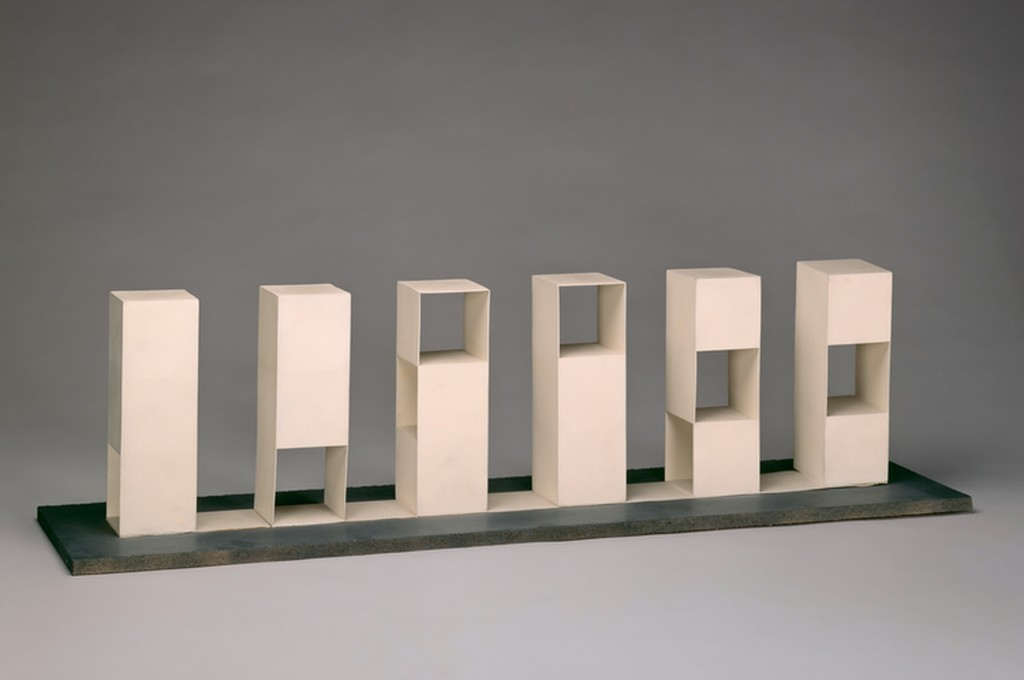
\includegraphics[width=4in]{Henry Thesis/Images/LeWitt_1-2-3}
\caption{\emph{Series 1-2-3: 47 3-Part Variations on Three Different Kinds of Cubes} (1968) by Sol LeWitt}
\label{fig:sol}
\end{centering} 
\end{figure}

Placing emphasis on the medium in minimal art often means the work is literal, and pieces are titled after the material they are made out of, if they are titled at all.\footnote{\cite{batchelorMinimalism1997}, 13.} The material remains unprocessed and unpainted and is more often than not an industrial product such as steel, glass or plastic. Carl Andre's \emph{144 Aluminum Square} (1967) shown in Figure \ref{fig:carl} is a perfect example of this concept.\footnote{\cite{andre144AluminumSquare1967}} One in a series of six sculptures, 144 twelve-inch squares of aluminum (or magnesium, lead, etc.) are assembled in a square on the floor to form the piece. \emph{144 Aluminum Square} engages an audience through its medium and placement. Visitors are allowed to walk over the sculpture and gain an understanding of the material through both visual and physical interaction.\footnote{\cite{144MagnesiumSquare}}

\begin{figure}[htbp]
\begin{centering} 
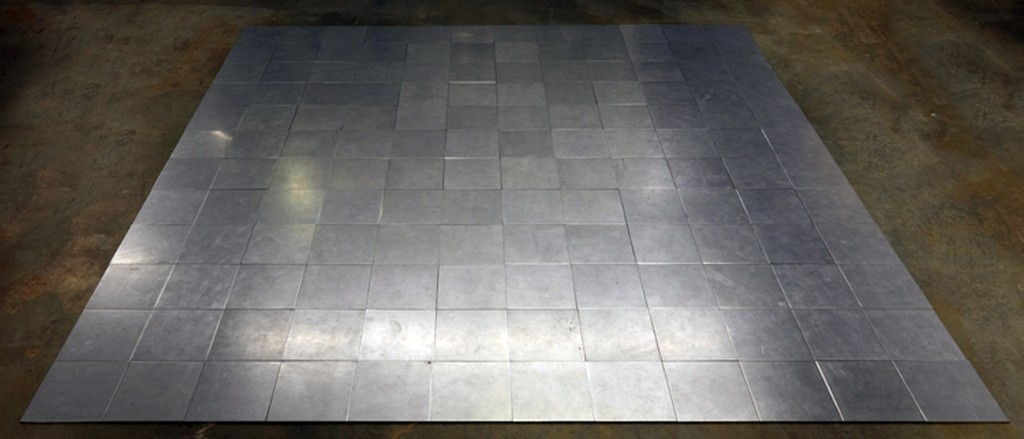
\includegraphics[width=4in]{Henry Thesis/Images/Andre_144Aluminum}
\caption{\emph{144 Aluminum Square} (1967) by Carl Andre}
\label{fig:carl}
\end{centering} 
\end{figure}

Techno also strays towards the literal in its naming conventions. Instruments produced by Roland in the early to mid 1980s are now part of what amounts to the canon of dance music and modifications of the names of these instruments have created a wealth of track titles. The sound of the Roland TR-909, TR-808, TB-303 and SH-101 are prized for their distinctive character and are key "materials" in electronic music production. Daft Punk's \emph{Revolution 909} celebrates the shuffle of TR-909 hi-hats, Tobias Von Hofsten's \emph{I Love My 808} centers the boom of the TR-808 bass drum, and Robert Hood's \emph{SH.101} for the cutting filter resonance of the SH-101.

\subsection{In Modern Classical Music}
Like their associates in the visual arts, the minimalist composers were typified by an emphasis on exploring simple concepts. Minimalist music came about as a response to the dominance of serialist techniques in the 1950s.\footnote{\cite{obendorfMinimalismDesigningSimplicity2009}, 42.} Serialists like Schoenberg, Babbitt and Boulez abandoned traditional tonal structures, favoring the procedural use of pitch collections.\footnote{\cite{Serialism}} Often working with an ordered sequence (series) using all twelves pitches, composition involved applying different transformations to the series. Careful listening to the series and transformations are often required to understand the piece as more than a chaotic spread of notes and rhythms. This complexity makes it difficult to appreciate for ears unfamiliar with the music. Instead of continuing to pursue complex musical transformations, minimalist composers made use of familiar harmony, rhythm and form.\footnote{\cite{potterMinimalismUSA2019}}

The groundwork of minimalism was laid by Terry Riley, Steve Reich, La Monte Young, and Philip Glass, who were also artists based in New York City in the 60s. Running in the same circles as minimal visual artists, the composers also rejected the label when it was applied to their work and early patrons of Steve Reich were artists Sol LeWitt and Richard Serra.\footnote{\cite{obendorfMinimalismDesigningSimplicity2009}, 40, 49.}

In composition, minimalists were preferential to repetition, phase shifting and musical processes. Phase shifting allowed for the creation of intricate and evolving music from a single motif. \emph{It's Gonna Rain} (1965) is a tape music piece by Steve Reich that began his exploration of phase shifting music. Composed using two tape loops of a preacher speaking, one of the loops is slowed down, causing the tapes to drift out of phase. The loops approach a round before returning to a brief moment in phase.\footnote{\cite{huizengaFiftyYearsSteve2015}} Reich's \emph{Clapping Music} (1972) used a different implementation of phasing, and like \emph{Piano Phase} (1967), it was written for live performers. Unlike the gradual phasing of \emph{It's Gonna Rain} and \emph{Piano Phase}, abrupt metric phase shifts in \emph{Clapping Music} creates a distinct collection of musical patterns.\footnote{\cite{morganAnthologyTwentiethCenturyMusic1992}, 435.}

Terry Riley experimented with series of patterns as well, focusing on the composition of small musical modules. Riley's \emph{In C} (1964) is the most influential example, which makes use of 53 modules. Written for any number of performers playing any instrument, \emph{In C} gives musicians the freedom to determine the form. Changes come when a performer chooses to advance to the next module, and can result in performances that last up to an hour and a half.\footnote{\cite{obendorfMinimalismDesigningSimplicity2009}, 42.}

Other avenues of minimalist composition removed any allowance for improvisation. Pieces of ``process music'' were written and played in a strict set of rules. In the 1968 manifesto ``Music As A Gradual Process'' Steve Reich laid out his concept of algorithmic composition. Process music determined ``all note-to-note details and the overall form simultaneously,'' which separated it from gradual, improvised composition.\footnote{\cite{reichWritingsMusic1974}, 11.} As Carl Andre's sculptures emphasized transparency, so too did process music. "I don't know any secrets of [the composition's] structure that you can't hear" said Reich on the form.\footnote{\cite{reichWritingsMusic1974}, 10.}

Philip Glass joined Reich in process music, making use of additive and subtractive processes. \emph{1 + 1} (1969) was a simple composition by Glass that was his first exploration in using a musical process. Using only rhythm, a player adds and subtracts rhythmic units, played by tapping on a table.\footnote{\cite{obendorfMinimalismDesigningSimplicity2009}, 47.} With \emph{Music In Twelve Parts} (1974) Glass expanded the language of additive processes across twelve pieces of music and twelve musical lines.\footnote{\cite{pageTwelvePartsPhilip}} In later years Glass began to find success outside of the academic music world, scoring for Hollywood soundtracks, which brought minimalist approaches to more ears.\footnote{\cite{evanstristanGlassPhilip}}

The commercial success minimalist composers achieved---Glass with \emph{Glassworks} (1982), and Reich's collaboration with Pat Metheny \emph{Electric Counterpoint}---came after the influence of their music had already started to effect popular music. In the 1970s tape and synthesizer experimentation grew beyond the academic realms of the minimalists, driven in no small part by Wendy Carlos. Her debut album \emph{Switched On Bach} (1968) rendered J.S. Bach on synthesizers, and was a wild success which made synthesizer technology common knowledge.\footnote{\cite{wendycarlosSwitchedOnBach1968}; \cite{prendergastAmbientCenturyMahler2000}, 70.} As synthesizer sales rose, other musicians began to intertwine minimalist concepts into electronic music.

Brian Eno was inspired by the minimalist composers and applied some of the techniques to create what he would call ``ambient.'' Eno's career in the earlier part of the 1970s was focused on art rock, but with \emph{Discreet Music} (1975) he began to create music that, in his words, ``could be listened to yet could be ignored.''\footnote{\cite{brianenoDiscreetMusic1975};\cite{enoDiscreetMusicLiner}} Inspired by Reich's ``Music As a Gradual Process,'' Eno built a tape echo system, into which he routed a synthesizer playing a sequence from Pachelbel's \emph{Canon in D}.\footnote{\cite{enoDiscreetMusicLiner}; \cite{prendergastAmbientCenturyMahler2000}, 119.} The canon plays quietly along with its echo, not much louder than the tape hiss. Where strict examples of process music ruled out interfering, Eno chose to make gradual adjustments to the synthesizer in recording. Doing so made "Discreet Music" a more improvised and performative kind of process music.

With \emph{Ambient 1 (Music for Airports)} (1978) Eno began to describe the gradual, meditative music he was making as ambient.\footnote{\cite{enoAmbientMusicAirports1978}} Outlining his intentions in the liner notes, Eno said he wanted to create ``environmental music suited to a wide variety of moods and atmospheres.''\footnote{\cite{enoMusicAirportsLiner}} Distancing himself from Muzak, the de-facto background music of the time, Eno emphasized that no musical compromises were necessary with ambient.\footnote{\cite{enoMusicAirportsLiner}; \cite{prendergastAmbientCenturyMahler2000}, 123.} The mission with ambient music was to create music that was ``able to accomodate many levels of listening attention without enforcing one in particular.'' \footnote{\cite{enoMusicAirportsLiner}}

In 1981, experimental musician and performance artist Laurie Anderson had a surprise UK number 2 chart hit with an eight-minute single, the minimalist \emph{O Superman (for Massenet)}. Anderson uses a constant, haunting, ``ha ha ha ha'' vocal pulse as the grounding motif of the piece. The music is in a tonal grey area, and furthering the piece's confusing ambience, Anderson processes her voice into strange robotic tones with a vocoder.\footnote{\cite{eckenrothOnceAgainMusic2014}} Inspired by a 19th century Massenet aria, the lyrics were written as a prayer to American authority and a critique of the deadly failures of the military in the Iranian hostage crisis.\footnote{\cite{davesimpsonHowWeMade2016}} Late in the piece, a synthesized string ostinato expands using an additive process, giving more similarity to other minimalist composers.\footnote{\cite{eckenrothOnceAgainMusic2014}}  By the late 1980s, minimalist techniques like those popularized by Anderson and Eno would begin to appear in electronic dance music.

\section{In House and Techno}

\subsubsection{E2-E4}

When German guitarist Manuel G{\"o}ttsching released his fourth solo album, \emph{E2-E4} (1984) he could not anticipate how it would influence the nascent genres of house and techno.\footnote{\cite{manuelgottschingE2E41984}} In the 1970s, G{\"o}ttsching was best known as the lead of Ash Ra Tempel, a group that made its name in psych-rock and synthesizer experimentation, before it became his solo project.\footnote{\cite{AshRaTempel}} G{\"o}ttsching recorded \emph{E2-E4} in 1981, three years before it would be released. He recorded it in one take, using guitar, a drum machine and two gentle chords he programmed on a synthesizer. The album was named for a common chess opening move and the open strings of a guitar.\footnote{\cite{d.straussManuelGottsching2006}} In the years that followed \emph{E2-E4}'s release, it brought minimalism into dance music with a slew of remixes and reinterpretations. 

In \emph{E2-E4} airy synth melodies bounce and mutate over the consistent repetition of the underlying chords. Rhythmic emphasis shifts as synthesizer envelopes expand and contract while echo and delay are used for gradual changes in mix that make for unmistakable similarities between G{\"o}ttsching's recording and Eno's ambient process music. While G{\"o}ttsching did not use pre-determined musical processes like the American minimalist composers, his improvisation with the repeating background material invoked the character of minimalism.\footnote{\cite{reichWritingsMusic1974}, 11.} To listen to \emph{E2-E4} evolve over the course of an hour is a hypnotic and entrancing experience. With a free structure anchored by a four-to-the-floor bass drum, the album fit in well with the eclectic musical taste of the post-disco club scene in New York.\footnote{\cite{lawrenceSaturdayMassLarry2014}}

G{\"o}ttsching's record was discovered by Larry Levan, the resident DJ at New York's Paradise Garage night club. Levan was known for his imaginative musical selections at the Garage, ranging from The Clash to The O'Jays, and he turned \emph{E2-E4} into a staple of the club.\footnote{\cite{lawrenceSaturdayMassLarry2014}} He often played the entire hour of the album uninterrupted in the early morning hours.\footnote{\cite{d.straussManuelGottsching2006}} Levan's selections also influenced the development of house music that was happening in Chicago and New York at the time. The New York variation of Chicago House, Garage House, is said to have taken its name from the sonic environment Larry Levan built at Paradise Garage.\footnote{\cite{reynoldsGenerationEcstasyWorld1998}, 35.}   

In 1989 Italian production outfit and record label D.F.C. (Dance Floor Corporation) caught on to \emph{E2-E4}'s club potency. The label licensed an eight-bar sample of \emph{E2-E4} from G{\"o}ttsching and took to the studio.\footnote{\cite{d.straussManuelGottsching2006}} D.F.C. reinforced the sample with a house rhythm, percussive piano chords and swirling synth arpeggios. Echoing bird calls, ocean sound effects, and breathy vocals in Spanish by Carolina Damas finished the record.\footnote{The bird call sample would also cement itself in dance music in 1989. For more: \cite{sherburneAnacondaPacificState2014}} Released as the eponymous single \emph{Sue{\~n}o Latino} it was an unabashed exotic re-interpretation of \emph{E2-E4}. ``Sue{\~n}o Latino'' took the club world by storm, charting number one on European dance charts.\footnote{\cite{d.straussManuelGottsching2006}} Alongside another 1989 dance hit, ``Pacific State'' by 808 State, ``Sue{\~n}o Latino'' defined the brief ``balearic beat'' conjuring images of warm Mediterranean beaches in Ibiza, Spain.\footnote{\cite{brewsterbillSearchBalearic2008}} Capitalizing on the track's success, a remix of ``Sue{\~n}o Latino'' was commissioned that brought \emph{E2-E4} in the creative hub of the Detroit electronic scene.

Detroit techno producer Derrick May made the ``Illusion First Mix'' of ``Sue{\~n}o Latino'' in 1992.\footnote{\cite{suenolatinoSuenoLatinoDerrick1992}} His remix removed almost all traces of the G{\"o}ttsching sample, instead reworking the piano parts with a new flute melody. When the sample does appear, it is edited so much that it's hard to pick it out in the mix. Another Detroit producer, Carl Craig, took a less subtle approach to using \emph{E2-E4}.

As ``Sue{\~n}o Latino'' did five years earlier, Craig's ``Remake Uno'' (1994) sampled significant portions of G{\"o}ttsching's improvisation. Craig emphasized the jazzier parts of the sample, adjusting it to play at a faster tempo and substituting shuffling jazz percussion in place of the original rigid drum machine.\footnote{\cite{paperclippeopleRemake1994}} Later that year a remix of ``Remake Uno'' called the ``Basic Reshape'' was issued on Craig's Planet E record label.\footnote{\cite{paperclippeopleRemakeBasicReshape1994}} ``Reshape'' distilled \emph{E2-E4} to its essence. Made by Berlin-based producers Mark Ernestus and Moritz Von Oswald, better known as Basic Channel, the remix brought \emph{E2-E4} back to Germany.\footnote{\cite{mcdermottLabelMonthBasic2018}}

Drawing on the studio techniques of dub reggae, percussion echoes through the Basic Channel remix, and low chords weave around the regular pulse of the kick drum and bass loop. Basic Channel ditched the samples that made previous remixes easy to trace back to the original recording, only leaving the arpeggiated bass riff. These drastic reductions made the remix almost more like the original \emph{E2-E4}. ``Basic Reshape'' mirrored the open and improvisation ready canvas that G{\"o}ttsching had composed the original \emph{E2-E4} for.

The movement of ``Remake Uno'' from Detroit to Germany was a common journey for electronic music to make in the 1990s. Unlike other rave scenes happening in the UK, Europe, and elsewhere in the United States, Detroit's techno scene was explicit in combining minimalist aesthetics with dance music. Their work would find resonances with musicians across the United States and Europe, leading to the rise of minimal techno.

\subsection{Minimized Techno}

\subsubsection{Belleville Three}
Techno is often defined by a synthesized musical arrangement, and like similar forms of dance music that appeared alongside it in the mid 1980s such as house, it is often driven by a four-to-the-floor kick drum. Unlike house, which draws on soul and disco, early techno drew upon the sounds of funk and electro, a synth infused strain of hip hop. The origins of techno can be traced to three friends who grew up just outside Detroit, in the small suburban city of Belleville. The ``Belleville Three'' of Juan Atkins, Derrick May\footnote{\emph{It is important to note that as of April 2021, Derrick May faces multiple sexual harassment and assault allegations, complicating his legacy in the techno scene.} \cite{rossSevenMoreDerrick2021}} and Kevin Saunderson would move to Detroit, and there they would find a scene eager for a futuristic vision of dance music.\footnote{\cite{reynoldsGenerationEcstasyWorld1998}, 15.} 

Paving the way for techno was the Detroit area radio show ``The Midnight Funk Association,'' hosted by The Electrifyin' Mojo, real name Charles Johnson. Credited with popularizing the sounds of electronic music among the youth of motor city, ``The Midnight Funk Association'' began broadcasting on WGPR Detroit in 1977.\footnote{\cite{zlatopolskyTheaterMindLegacy2015}} With a nightly show free from the restraints of commercial formatting, he played selections that spanned a range from Parliament Funkadelic to The B-52s and beyond. Mojo championed the music of synth-pop innovators Prince and Kraftwerk, playing full albums and rare B-sides. ``You’d sit there in a trance waiting for each record Mojo was going to play,'' said Juan Atkins.\footnote{\cite{zlatopolskyTheaterMindLegacy2015};\cite{reynoldsGenerationEcstasyWorld1998}, 16.} The impression ``The Midnight Funk Association'' left on Atkin's taste was also true for the club scene in Detroit, where Atkins began DJing under the name Deep Space Soundworks.\footnote{\cite{reynoldsGenerationEcstasyWorld1998}, 17;\cite{sickoTechnoRebelsRenegades2010}, 43.}

In 1981 Juan Atkins and Rick ``3070'' Davis released an electro track under the name Cybotron, called ``Alleys of Your Mind.''\footnote{\cite{cybotronAlleysYourMind1981}} The single became a local success thanks to airplay support from The Electrifyin' Mojo.\footnote{\cite{zlatopolskyTheaterMindLegacy2015}} Cybotron releases carried futurist visions, while drawing on the industrial history of Detroit with tracks like ``Cosmic Cars'' and ``Techno City.''\footnote{\cite{reynoldsGenerationEcstasyWorld1998}, 18.} Cybotron would sign to San Francisco based Fantasy for an album in 1983, and after three singles for the label Atkins left the group in 1985. Starting his own label, Metroplex, Atkins' first solo release was ``No UFO's'' as Model 500.\footnote{\cite{model500NoUFO1985}} ``No UFO's'' exchanged the breakbeat of electro for a regular bass drum pulse, without losing any futuristic funk. Metroplex also became platform for releases from Kevin Saunderson, Derrick May and newcomer Eddie Fowlkes, who the trio had met in Detroit. Two years after the first Metroplex release, each member of the Belleville Three had established his own record label, Saunderson with KMS (Kevin Maurice Saunderson) and May with Transmat. 

Over in Chicago, the growing house music scene was attracting attention from British and European record labels. A{\&}R scouts searching for talent realized that records coveted by Chicago DJs were being produced by musicians in Detroit.\footnote{\cite{reynoldsGenerationEcstasyWorld1998}, 23.} Neil Rushton, an A{\&}R for Virgin Records, saw potential in the Detroit sound, and began to work on assembling a compilation.

Announcing techno to a British audience was the 1988 compilation album \emph{Techno! The New Dance Sound Of Detroit.}\footnote{\cite{sickoTechnoRebelsRenegades2010}, 66;\cite{variousartistsTechnoNewDance1988}} The album gave a name to the music, taking the term "Techno" from Juan Atkin's tracks ``Techno Music'' and ``Techno City'' (1984).\footnote{\cite{sickoTechnoRebelsRenegades2010}, 68;\cite{cybotronTechnoCity1984}} Released on Virgin Records imprint 10 Records and curated by Rushton and Derrick May, it licensed music from the foundational labels Metroplex, Transmat, and KMS. Kevin Saunderson, working under the name Inner-City, contributed the pop-leaning ``Big Fun'' to the compilation, which charted in the UK Top 40 as a single.\footnote{\cite{sickoTechnoRebelsRenegades2010}, 68.} The album brought international success to the Belleville three,  who were soon wrapped up in album negotiations, tours and remixes.\footnote{\cite{sickoTechnoRebelsRenegades2010}, 71-72} With Atkins, May and Saunderson now pursuing opportunities outside of Detroit, they left a space in the scene that would be filled by new voices.

\subsubsection{Underground Resistance}

With the appearance of Underground Resistance in 1990, the second wave of Detroit techno began to materialize. Operating as a faceless collective, the label was more militant and ideological than labels that came before it. Founded by Jeff Mills and Mike Banks, they sought to fix the problems they felt increased commercialism brought to the Detroit scene.\footnote{\cite{schmidtJeffMillsLecture1998a}} At the time Mills was best known as ``The Wizard'' on WJLB Detroit. DJing with three turntables and a drum machine, his three hour sets neared the influence of The Electrifyin' Mojo.\footnote{\cite{schmidtJeffMillsLecture1998a};\cite{broughtonInterviewJeffMills2017a}} Mills also produced a few industrial records as Final Cut, where he met studio musician Mike Banks in recording sessions.\footnote{\cite{sickoTechnoRebelsRenegades2010}, 99.} The label and collective grew larger, and artists like Carl Craig, Robert Hood and Drexciya were among the new talent that Underground Resistance supported.

The sound of the label was more intense than the radio friendly techno present on the \emph{Techno!} album too. Leaving behind pop song structures, Underground Resistance leaned in the direction of late 80s electronic-punk styles like industrial and EBM (``Electronic Body Music'') popularized by groups like Nitzer Ebb, Front 242 and Meat Beat Manifesto.\footnote{\cite{reynoldsGenerationEcstasyWorld1998}, 220.} The influence of industrial made their style of techno more repetitive and hardcore, with hard-edged synths and relentless drums that matched the aesthetics of the label.

Underground Resistance did not shy away from political engagement either. With releases like \emph{Acid Rain}, and \emph{Riot} UR addressed the social, environmental and political realities that faced Black people in Detroit. \emph{Message To The Majors} (1992) targeted critiques at both the Detroit Police Force and major record labels. "Message to all murderers on the Detroit Police Force - We'll see you in hell!" read the release's artwork, as seen in Figure \ref{fig:messagetothemajors}. A sample from EPMD's track "Crossover," which critiqued pop crossovers in hip hop, was looped over the beat.\footnote{\cite{undergroundresistanceMessageMajors1992a}} Releases of this kind lead to favourable comparisons with hip hop group Public Enemy and set UR apart from other dance labels.\footnote{\cite{sickoTechnoRebelsRenegades2010}, 100.}

\begin{figure}[htbp]
\begin{centering} 
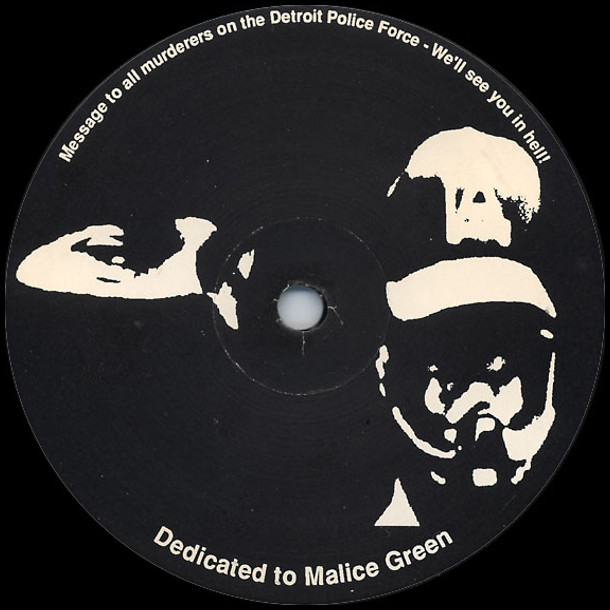
\includegraphics[width=3in]{Henry Thesis/Images/message_to_the_majors}
\caption{Art from Underground Resistance - \emph{Message To The Majors} (1992)}
\label{fig:messagetothemajors}
\end{centering} 
\end{figure}

The label fought against convention in more unusual ways as well. Numerous Underground Resistance releases were cut so the music played from innermost groove of the record to the outside. Other releases were interspersed with locked groove loops that distilled techno down to endless repetitions of one-bar sequences.\footnote{\cite{x-102OBXA1992}} These locked grooves came alive in the hands of a DJ like Jeff Mills who could use them as modular form of composition in his DJ sets.

Popularity in the international underground took Underground Resistance by surprise in 1991 when New York DJ and producer Joey Beltram called to tell them just how nuts a crowd in Germany had gone for the track ``Elimination.'' Mills recalled in 1998 how surprising it was to get Beltram's call, ``We didn't have a clue what was going over here [in Germany]. We had heard some things from Kevin [Saunderson] about what a rave was, you know, 10,000 people, but we didn't know.''\footnote{\cite{schmidtJeffMillsLecture1998a}} The popularity of Underground Resistance in Germany resulted in a few licensing deals with the Berlin based Tresor label, which released Mills' first solo album.

\emph{Waveform Transmission Vol. 1} (1992) was a landmark in bringing the brutal and minimal techno sound Mills was working on to a wider audience. Tracks like ``Phase 4'' (a remix of a German techno hit ``Der Klang Der Familie'' by Phase 3) and "Berlin" were two distorted industrial techno freak-outs that set a high bar for material to follow. Underground Resistance's work with Tresor also strengthened ties between the growing German techno scene and Detroit. Mills would return with the third installment of the \emph{Waveform Transmission} series. In the interim \emph{Waveform Transmission Vol. 2} was recorded by The Vision, otherwise known as fellow Underground Resistance member Robert Hood.

Hood would release one of the defining albums for Detroit techno in 1994 with \emph{Minimal Nation} and it became a manifesto for a growing minimal aesthetic. Initial plans to call the album \emph{Access Authorized Repetition}, a title which emphasized the power of repetition in techno, were scrapped when Hood observed to Mills that ``the minimal nation is rising.''\footnote{\cite{holbenMakingMinimalNation2019}} DJs were quick to pick up early pressings of the album too, a sign that Hood's observation was correct. ``People were excited about this record. Immediately I knew there was something special about this record, that it was different,'' recalled Hood in an interview.\footnote{\cite{holbenMakingMinimalNation2019}} The sound of the album was unprocessed and direct, due to the limited studio equipment he was working with.\footnote{\cite{holbenMakingMinimalNation2019}} Robert Hood followed up \emph{Minimal Nation} with \emph{Internal Empire} (1994) for Tresor. Hood's intention with minimalism was not to build interest through changes but with ``rhythms inside of rhythms inside of rhythms.''\footnote{\cite{burnsRobertHoodLecture2014}} With tracks like ``Minus'' on \emph{Internal Empire} Hood used phasing rhythms not unlike those of Steve Reich, creating a hypnotic atmosphere.

The discovery that drove the repetitive, minimalist techno, was that when techno refrained from change, it was able to incite a change in an audience. Again speaking in 1998, Jeff Mills reflected on how he and Robert Hood approached the concept and its use in the context of a club.

\begin{quote}
   We discussed the idea of, in terms of time, how long it takes for the people to really get excited listening to the same sequence over and over again. It was about two-and-a-half to three minutes. If you put the needle at the beginning of a record and you just simply let it play and you stand back, somewhere within that time frame, someone’s going to scream, because the music, it just doesn’t change. And because you know that it doesn’t change you become more relaxed. And if you become more relaxed, then you know that you can move your body much better if you don’t know what to anticipate. It brings this excitement.\footnote{\cite{schmidtJeffMillsLecture1998a}}
\end{quote}

In this situation, the DJ becomes an operator in a push and pull dynamic, deciding how long dancers can be familiar with the track. Once the excitement of the familiar is reached, it can be replaced with the excitement of difference. Mills and Hood could allow dancers to reach a trance-like state and then pull them out of it. With minimalism Hood wanted to ``have that one guy in the back of the room just lose it and just start to scream and almost catching the holy ghost. That was my whole focus.''\footnote{\cite{burnsRobertHoodLecture2014}} Others in the techno scene also began to see the potency of heightened repetition as a powerful tool in dance music. From 1993 onward an increasing number of artists inside and out of Detroit began to release techno that built upon this concept.

\subsection{Further Reductions}

\subsubsection{Plastikman}

Richie Hawtin became another key player in the minimal techno sound, coming from Windsor, Ontario, just across the lake from Detroit.\footnote{\cite{reynoldsGenerationEcstasyWorld1998}, 225.} Active since the late 80s as DJ, he ran somewhat in the same circles as the Underground Resistance crew. In 1990 Hawtin founded Plus 8 Records with fellow Canadian DJ John Acquaviva. His first release on the label was \emph{Elements of Tone} as States of Mind, a record that drew upon the bass heavy UK ``bleep'' techno sound.\footnote{\cite{statesofmindElementsTone1990}} After a string of releases, in groups and solo, Hawtin started releasing music under the name Plastikman, which became his most influential project.

Plastikman began in 1993 with the album \emph{Sheet One} and two singles, the percussion-focused \emph{Spastik} and the slowly mutating \emph{Krakpot}.\footnote{\cite{plastikmanSheetOne1993};\cite{plastikmanSpastik1993};\cite{plastikmanKrakpot1993}} The production process for Plastikman records was as elastic as ``plastik'' implied. Similar to Manuel G{\"o}ttsching improvising \emph{E2-E4} Hawtin improvised with his synthesizers for over an hour at a time and edited down the final results to fit on a record.\footnote{\cite{burnsRichieHawtinLecture2013}} 

As a relative outsider to the tight knit Detroit scene, Hawtin saw his early work as an attempt to fuse his inspirations, the futuristic techno of Detroit and the hypnotic acid house of Chicago.\footnote{\cite{burnsRichieHawtinLecture2013}} Hawtin was not the only one involved in the the Detroit scene to be inspired from afar. In Germany, where Detroit techno was finding a strong audience, the duo Basic Channel began to expand upon the sound by melding it with production techniques from dub-reggae.

\subsubsection{Basic Channel}
Moritz Von Oswald and Mark Ernestus began the Basic Channel record label in 1993, the same year Hawtin began the Plastikman project. The records they would release, under a variety of psuedonyms---Cyrus, Maurizio, Quadrant, Basic Channel---would become fundamental in creating dub-techno. With dub-techno, the music was inclined toward gestural use of echo, delay, and reverb, rather than melody. Combining space-filling studio effects common in reggae and dub music with synthesizers and drum machines, and an inclination for repetition, Basic Channel brought new sonic dimensions to techno.

Von Oswald and Ernestus were not strangers in techno, having built strong connections with the Detroit scene in the years prior. In 1989 Ernestus opened the record store Hard Wax, which became the primary German importer of Detroit techno.\footnote{\cite{mcdermottLabelMonthBasic2018}} Moritz Von Oswald was already producing techno prior to Basic Channel. With fellow ex-Palias Schaumberg band member Thomas Fehlmann, Von Oswald put out several releases as 2MB aka ``2 Men in Berlin.''\footnote{\cite{2MB}} Collaborations with Detroit techno originators Juan Atkins and Eddie Fowlkes lead ``3 Men in Berlin'' releases as well.\footnote{\cite{3MB};\cite{fehlmannTimetable}}

The first Basic Channel release was the searing ``Enforcement'' (1993).\footnote{\cite{cyrusEnforcement1993}} The original mix of \emph{Enforcement} clocked in at 150 beats per minute and lasted just over thirteen minutes. A relentless and brutal track, as Figure \ref{fig:enforcement} attests, it was a clear nod to the intensity of Underground Resistance. Jeff Mills was brought on to provide the \emph{Mills Mix} remix on the B-side. After \emph{Enforcement}, delay effects started to become a larger part of the Basic Channel palette. Cascading chords echoes were central to ``Phylyps Trak,'' ``Lyot Rmx'' and ``Q 1.1.''\footnote{\cite{basicchannelPhylypsTrak1993}; \cite{basicchannelLyotRmx1993}; \cite{basicchannelQ111993}} Restraint in the use of echo was of equal importance, in order for every instrument to hold a place in the cavernous soundscape.

\begin{figure}[htbp]
\begin{centering} 
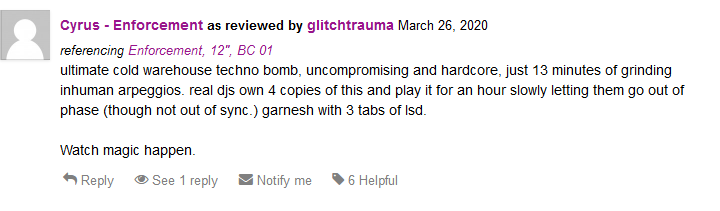
\includegraphics[width=5in]{Henry Thesis/Images/enforcement_review}
\caption{Discogs review of \emph{Enforcement}}
\label{fig:enforcement}
\end{centering} 
\end{figure}

The B-side of \emph{Inversion} (1994), ``Presence'' is the most unusual of the Basic Channel releases. In the track a synth plays in counterpoint with an echo for 20 minutes. ``Presence'' stands out as having a more direct connection with early ambient recordings than beat-driven techno.\footnote{\cite{cyrusInversion1994}} Not only was it an odd piece of music for a techno label, it also featured the inside-out playback trickery that Underground Resistance used. This was the work of National Sound Corporation (NSC), a record store turned mastering studio that catered to the needs of the Detroit producers and was adept at making unusual records. Basic Channel's work with NSC also showed how connected they were to the Detroit scene.\footnote{\cite{sickoTechnoRebelsRenegades2010}, 109-110.}

The abstract quality of Basic Channel extended to their mysterious label art, which was void of almost all identifying information. With each successive release on the label the circle-wrapped logo was processed to beyond legibility. Eventually it became only understandable as a symbol of the label, as figure \ref{fig:bclogo} demonstrates.

\begin{figure}[htbp]
\begin{centering} 
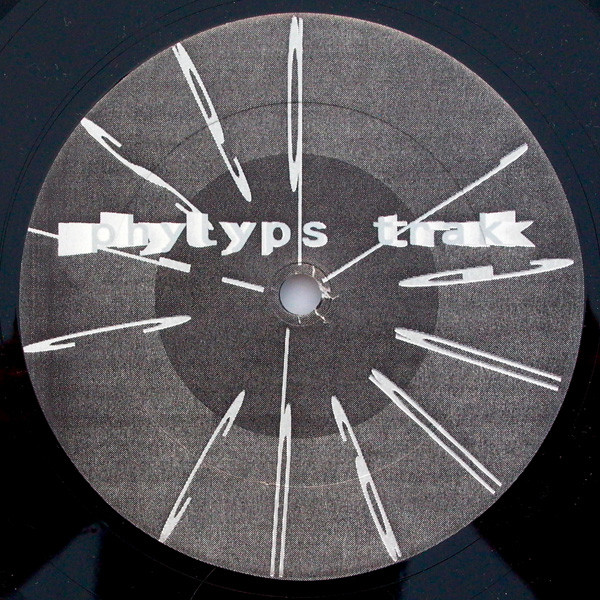
\includegraphics[width=2in]{Henry Thesis/Images/phylyps_trak}
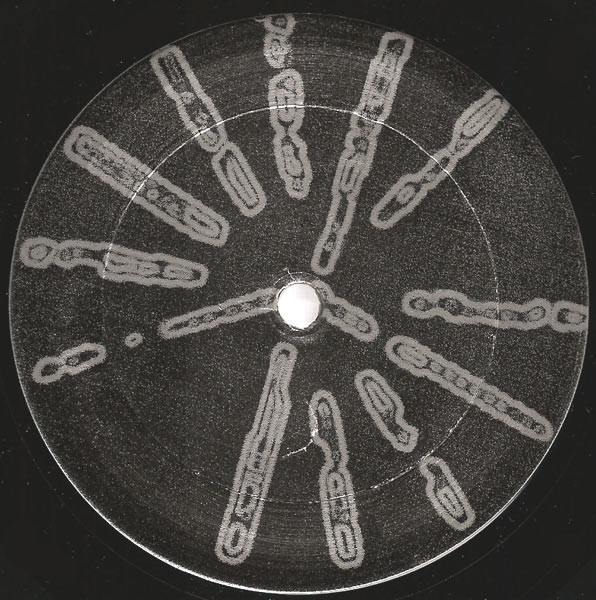
\includegraphics[width=2in]{Henry Thesis/Images/phylyps_trak_ii}
\caption{Changes to the Basic Channel logo between \emph{Phylyps Trak} (1993) and \emph{Phylyps Trak II} (1994)}
\label{fig:bclogo}
\end{centering} 
\end{figure}

This trend of either untitled or barely--named music became commonplace in minimal techno. It followed the material transparency that minimalist sculptors used, with the sound was presented without commentary. It encouraged the listener to understand the music on their own terms, like one would approach a copper square in an art gallery. As described by the contemporary 90s techno group Global Communication, ``names tend to bias the listener by pre-defining images'' and a lack of prompting ``gives the listener the freedom of imagination.''\footnote{\cite{globalcommunication76141994}}

Ending the Basic Channel releases in 1994 with ``Phylyps Trak II,'' Von Oswald and Ernestus began to focus more on reggae.\footnote{\cite{basicchannelPhylypsTrakII1994}} The Rhythm {\&} Sound project embraced reggae and techno production aesthetics in equal measure. Chain Reaction, a successor label to Basic Channel was also established. With the new, Basic Channel helped encourage the growth of minimal and dub-techno in the latter half of the decade.\footnote{\cite{maya-roisinslaterGerhardBehlesRobert2016}}

\subsubsection{Monolake}

Monolake began as a collaboration between Robert Henke and Gerhard Behles, releasing \emph{Cyan} (1996) on the Chain Reaction label.\footnote{\cite{monolakeCyan1996}} After two more singles, Henke and Behles released an album, \emph{Hongkong} (1997), named for field recordings they had collected in Hong Kong.\footnote{\cite{monolakeHongkong1997}} Compared with the whispering tape-noise of Basic Channel, Monolake brought a digital sound to the label. For that matter, Henke and Behles often saw themselves as programmers rather than musicians. They started Monolake while studying computer science in Berlin, and found themselves in the gap between techno and academic computer music.\footnote{\cite{maya-roisinslaterGerhardBehlesRobert2016}} The difference between the two worlds was striking as Henke explains it: 

\begin{quote}
On one side the music was only possible at institutions with big computers running overnight to create one minute of sound and, on the other, you had a young, sweaty Richie Hawtin at Tresor with a 909, 808 and a cheap effects unit.\footnote{\cite{burnsMonolakeSoundScientist2012}}
\end{quote}

The division between the technologies of academic music and club music began to dissolve as personal computers became more and more powerful. Monolake began to use the Max music programming language in their production process, and it soon replaced their analog hardware.\footnote{\cite{maya-roisinslaterGerhardBehlesRobert2016}} Using computers more, in order to perform on stage with laptops, Behles and Henke needed software that would allow them to play and manipulate audio loops. This led to the beginning of the development process for what would become the digital audio workstation Ableton Live.\footnote{\cite{maya-roisinslaterGerhardBehlesRobert2016}}

The initial prototype of Ableton was used on the albums \emph{Interstate} (1999) \emph{Gravity} and \emph{Cinemascope} (2001) before the official release in late 2001. Henke left the company in 2011 to focus on Monolake while Behles remained as the CEO.\footnote{\cite{maya-roisinslaterGerhardBehlesRobert2016}} Coming full circle with the electronic explorations in the 60s, the minimal techno artists found themselves pushing the technology of the late 1990s to fit their needs.

\subsubsection{Gas}
Wolfgang Voigt is another German producer who made substantial contributions to the development of minimal techno. Like Basic Channel, Voigt released under a number of aliases, notable among them is the ambient-techno he releases under the name Gas.\footnote{\cite{bacherWolfgangVoigt2018}} His first album as Gas, \emph{Gas} was released in 1996 followed by \emph{Zauberberg} (1997), \emph{K{\"o}nigsforst} (1999) and \emph{Pop} (2000).\footnote{\cite{gasGas1996};\cite{gasZauberberg1997};\cite{gasKonigsforst1999};\cite{gasPop2000}}

Beginning with \emph{Zauberberg}, the albums took on a conceptual theme informed by the forests around his home in Cologne, and the time he spent there while on LSD as a teenager.\footnote{\cite{mattfulkersonInterviewWolfgangVoigt2016};\cite{betaGasAmbientTechno2018}} Time-stretched loops from classical recordings from the likes of Wagner and Schoenberg are layered to create brooding ambient atmospheres.\footnote{\cite{betaGasAmbientTechno2018}} As Eno applied process music to Pachelbel's \emph{Canon in D}, Voigt made use of digital sampling technology often to manipulate his source material beyond recognition. The small repeating musical loops, and the sonic density of the Gas albums make the music an experience in both maximalism and minimalism.

Working around the single restraint of a bass drum, Voigt granted himself significant space for exploration. ``Everything was circulating around a straight bass drum. That was the common denominator, which was non-negotiable, otherwise there were no boundaries,'' and in the dense textures of the Gas albums, the bass drum often tangible connection to techno that remains.\footnote{\cite{bacherWolfgangVoigt2018}}

\subsubsection{DeepChord}
Dub-techno wound its way back to Detroit, where Rod Modell and Mike Schommer would carry the sound further as DeepChord. They set up the DeepChord label in 2000 when plans to release on Hawtin's Plus 8 label folded.\footnote{\cite{russellDeepChordDoesnCare2014}} In a busy first year the two released 8 singles, \emph{dc07} through \emph{dc14}, and the first DeepChord album, \emph{DeepChord 01-06}.\footnote{\cite{DeepChordDiscogs};\cite{deepchordDeepChord01062000}}

Encased in whispering washes of noise and low chord stabs, early DeepChord moved at a glacial pace, save for the drive of the kick drum. Repetition and gradual change were even more important to DeepChord records than the minimal techno that had come before.  By avoiding substantial change they heighten the effect of even the smallest adjustments. For ten minutes the A-side of \emph{dc11} remains in a valley of echoing synthesizer chords, before a gentle hi-hat appears on the off-beat.\footnote{\cite{deepchordDc112001}} It gives just enough alteration to add substantial rhythmic energy to the record.

Obsessed with repetition, Rod Modell describes working on DeepChord more like ambient composition. ``With many DeepChord tracks (DeepChord 10 comes to mind), I would drop out the percussion and let the loop go for days around the house.''\footnote{\cite{TenQuestionsDeepchord2007}} After Mike Schommer left the project in 2002, Modell began to shift DeepChord away from a synthesis forward sound to one that was more field recording focused. With the most recent DeepChord releases, Modell has taken to weaving processed ambient recordings into the soundscapes washing over the rhythms. The use of field recordings embodies the revelation Brian Eno encountered when he began to see the potential of music ``as part of the ambience of the environment, just as the color of the light and the sound of the rain were parts of that ambience.''\footnote{\cite{enoDiscreetMusicLiner}}

\section{Conclusion}

All of these artists have made contributions to minimalism, and certain components of the minimalist aesthetic have carried through the thirty--year history. Recognizing these shared concepts is valuable to understanding techno in more detailed musical analysis. 

The use of repetition is a significant part of minimalist form, giving scale and form to a work. In minimalist art the repetitions are often static or staggered, with little room for fluid change across repeated figures. Music can more easily apply changes across repetition: a rhythmic figure will repeat where a pitch can change. Phasing music can re-contextualize the repetition of a sequence to give the impression of difference and polyphony.

Repetition that changes through a process or effect is at the core of techno. Process music, as introduced by Steve Reich was static, and the application of performance and improvisation onto the process by Eno, G{\"o}ttsching and many other musicians is an important differentiation. Changing timbre, mix, and effects can sustain interest across a static rhythm or melody.

Reduction appears in every stage of minimalism discussed in this chapter. In art, the use of industrial materials is a reduction of the process otherwise applied in sculpture. The simplified tonal language preferred by minimalist composers was a rejection of the complexity in post-tonal music. Techno producers and the minimalist composers both work toward the reduction of pattern complexity and phrase sizes. In the next chapter, these concepts will be examined in practical musical applications. Through the analysis we can better understand the specific minimalist techniques and concepts implemented in techno.

\chapter{Analysis}

\section{Overview}

Understanding how minimalist concepts have interacted with techno, the following chapter applies this knowledge to analyze three recordings. These pieces demonstrate concepts that are, in my opinion, important in the creation of energizing and inspiring dance music. The examples are personal favorites, and not all are explicit ``minimal'' techno. As a result, the pieces can showcase how widespread minimalist techniques are in techno as a whole. I also want to stress the importance of listening to, or physically experiencing, the recordings. Literary descriptions of unfamiliar sounds are often less meaningful than the experience of the sound on the body, whether through auditory or other senses.\footnote{At the time of writing in April 2021, all three examples are available for listening online, however ``Lost In Space'' is currently only available on YouTube.} Experiencing the music also gives depth and complexity to otherwise stagnant transcriptions and diagrams.

I have split the chapter into three sections, each focused on a different piece and expressive technique. Analysis of ``Krakpot'' by Plastikman opens discussion of timbre and live mixing as an expressive tool. ``Lost In Space'' by Subsonic expands the expressive palette further using changes in instrumentation, structure, and dynamics to shape tension. The last piece, ``Phylyps Trak'' by Basic Channel, pushes against the clarity of form in the two other examples, bringing irregularities and unexpected changes to the palette.

\section{Timbre and Mix: ``Krakpot'' by Plastikman}
\label{sec:krakpot}

\subsection{Background}

Gradual adjustments in timbre, volume and spatial effects are critical to sustaining interest in techno music, as discussed briefly in Chapter 1. These types of adjustments allow drastic changes to the character of the sound, while leaving fundamental pitch and rhythmic content intact. This means one-bar loops can hold the listener's attention over a longer period of time than they might otherwise. ``Krakpot'' by Plastikman, aka Richie Hawtin, is an exceptional demonstration of how important gradual adjustments are in creating continuous intrigue over an otherwise static loop.\footnote{\cite{plastikmanKrakpot1993}}

\subsection{Instrumentation and Patterns}

``Krakpot'' measures in at just over eleven minutes long, with a tempo of 130 beats per minute, and spartan instrumentation consisting of a bass synthesizer and a drum machine. Meanwhile delay and reverb effects lend movement and depth to the piece. The Roland TB-303 bass synthesizer and Roland TR-707 drum machine used on the recording are pieces of gear from the 1980s whose sounds are identifiable in an instant.\footnote{\emph{See the following videos for demonstrations of the two instruments--} \cite{deathbydinsyncRolandTB303HQ2016}. \cite{zibbyboneRolandTR707Factory2017}.}  These pieces of gear give an unusual character to the track, in both sound and composition. To understand how ``Krakpot'' works, I will discuss how the TR-707 and TB-303 are used by Hawtin to guide the process of composing and recording a piece.

\subsubsection{Roland TB-303}

The relentless resonance, slides and accents unique to the Roland TB-303 are apparent from the first beat of ``Krakpot.'' As the track progresses, the TB-303 moves through constant sonic mutations, a feature which has made the small synthesizer a staple of club music since the late 80s. The TB-303 was released by the Roland Corporation in 1982, targeted at guitarists and bands looking for a futuristic budget synthesizer.\footnote{\cite{reynoldsGenerationEcstasyWorld1998}, 31.}  Roland designed the monophonic TB-303 with two oscillators options, a nasal saw wave and a softer square wave. A simplified keyboard on the front panel allowed for input of melodic sequences up to 64 steps long, as shown in Figure \ref{fig:tb303}. Going beyond sequencing pitch and time, slide and accent parameters enhanced dynamic possibilities of the sequencer, which reached closer to the performance and groove of a human bassist.

\begin{figure}[htbp]
\begin{centering} 
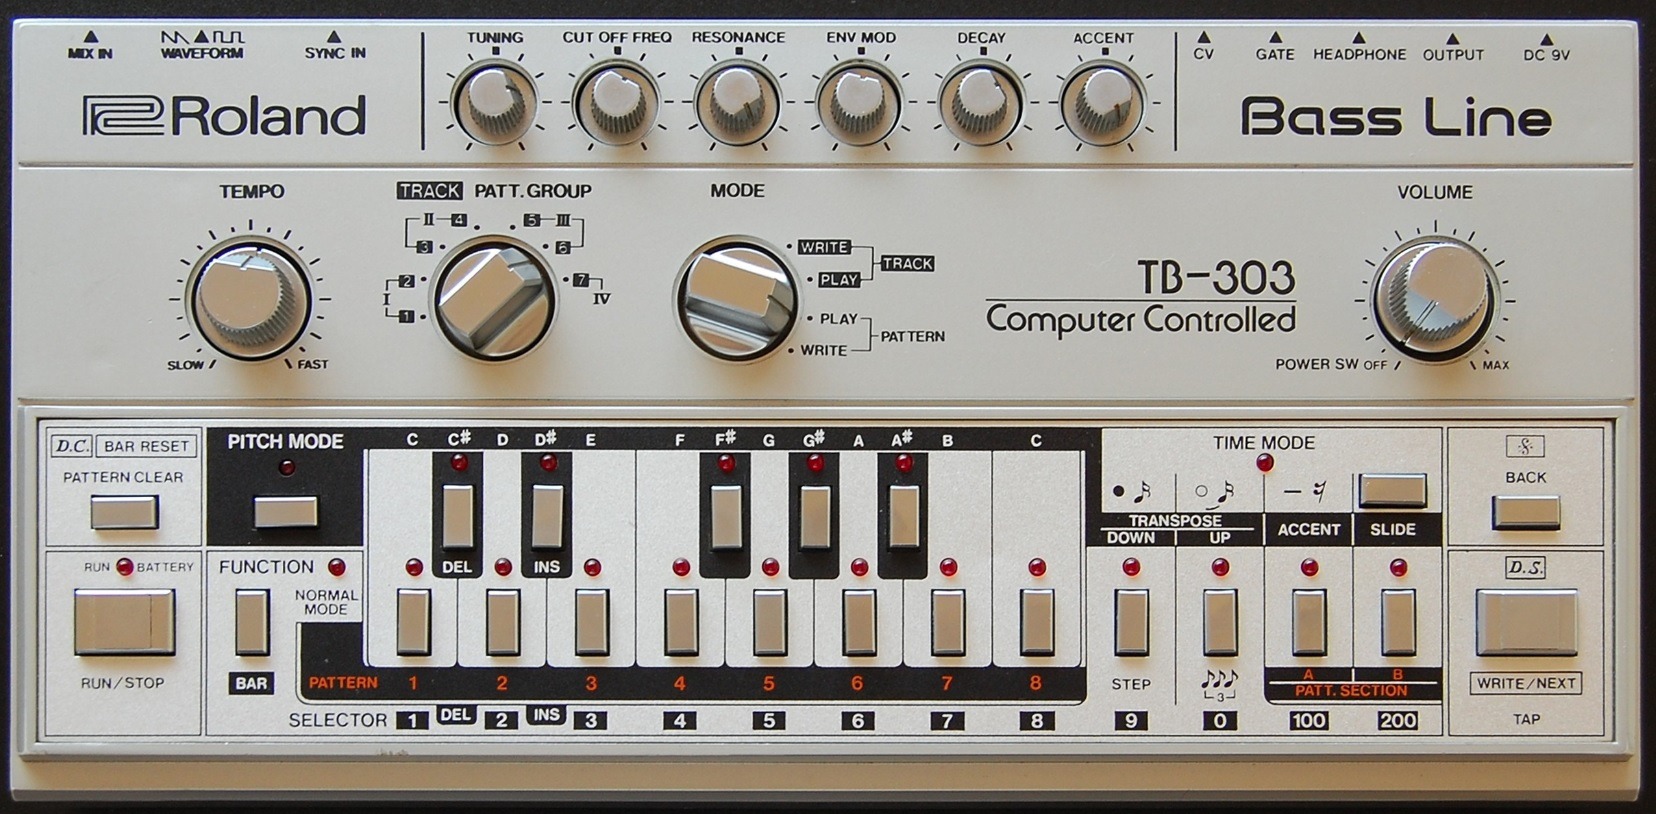
\includegraphics[width=5in]{Henry Thesis/Images/Roland_TB-303_Panel}
\caption{Roland TB-303 Front Panel}
\label{fig:tb303}
\end{centering} 
\end{figure}

The six knobs on the front of the TB-303 are its most important feature, and offer control of the synthesizer's sonic character.\footnote{\cite{simsRolandTB303Panel2008}} With these knobs the synthesizer became a playable instrument in the hands of many DJs, far more than just a programmable box.

On the far left of the panel is a general tuning knob, familiar to any musician. The second and third left-most knobs, filter cut-off frequency and resonance, are the most important to the sound of the TB-303. With a high resonance, the TB-303 emphasizes the harmonics of the square and saw wave, reshaping the sound. As the filter cut-off frequency is moved from low to high, higher harmonics become audible and the sound brightens. The three knobs on the right adjust the envelope of the filter. Envelope modulation controls how much the filter frequency is modulated by the envelope, and decay changes how quickly the envelope tapers off. Finally, the accent parameter changes how much louder an accented step is, and how much an accented step changes the filter envelope.\footnote{\cite{RolandTB303Owner1981}, 34.}

While Roland had no intention of making the ``Transistorized Bass''-303 sound like a real bass guitar, emphasizing the unique portamento (slide) and elastic character in marketing copy, it was unappealing to the guitarist market it sought to tap into.\footnote{\cite{ravalRolandTB303Not2020}} The little plastic box was difficult to program, and often resulted in mistakes and imperfect loops.\footnote{\cite{reynoldsGenerationEcstasyWorld1998}, 32.} The sequencer was confusing, stipulating that pitches be input first, followed by rhythm and performance effects.\footnote{\cite{RolandTB303Owner1981}, 5.} Production ended in 1984, and the TB-303 started to appear in second-hand stores. From these second-hand stores, house producers in Chicago picked up the box on the cheap. The The TB-303's combination of unpredictable programming and surreal bass sounds, became a valued feature in the hands of producers Marshall Jefferson, Herb Jackson, Spanky and DJ Pierre. In 1987, the four recorded ``Acid Tracks'' under the name Phuture.\footnote{\cite{reynoldsGenerationEcstasyWorld1998}, {32}.} Gradually adjusting the filter, they created a hypnotic house track that squeezed a resonant funk from the TB-303. ``Acid Tracks'' became the foundation of the ``Acid House'' genre, which spread the sound of the little Roland TB-303 throughout the club-sphere.\footnote{\cite{reynoldsGenerationEcstasyWorld1998}, {33}.} The timbral adjustments on the TB-303 by Phuture inspired countless other producers who began to record with it in a similar fashion. Plastikman follows in the tradition of using the TB-303 as an instrument performed with gradual filter modulation. The TB-303 was centered in Plastikman recordings, as ``it was always the one sound that didn’t sound like anything you’d ever heard.''\footnote{\cite{reynoldsGenerationEcstasyWorld1998}, 228.}


\subsection{Timbral Expression}

 The TB-303 is programmed to one melodic loop for the entire duration of ``Krakpot.'' The riff, transcribed in Figure \ref{fig:krakpotbass} is centered around A, with two accented slides up to G at the end of the bar. The bass functions in a rhythmic, rather than melodic role, with no indication of tonality given other than A and G, the interval of a minor seventh. Eighth-notes and accented glides syncopate the TB-303 against the bass drum, which maintains rhythmic interest in sections like 0:00 to 4:22 where the bass drum and TB-303 are the only active elements. The resonance and filter movement of the TB-303 is amplified further through in interactions with delay and reverb effects.


\begin{figure}[htbp]
\begin{centering}

\includegraphics[width=6in]{Henry Thesis/Images/Krakpot_bass2}
\caption{Transcription of the TB-303 on ``Krakpot'' with bass drum}
\label{fig:krakpotbass}
\end{centering} 
\end{figure}

The TB-303 is mixed with a long reverb that places it into the space of a virtual cavern. The reverb echoes are most prominent at moments of high resonance like at 3:54. The filter resonance creates reverberant ``ghosts'' that trail off, giving the impression of additional melodic content. When the filter resonance is at a highest setting, lower frequencies of the TB-303 begin to vanish and the sound fits into the mid-range of the frequency spectrum, as at 3:27 and 7:22. As resonance decreases, the bass gains more body and returns to the lower frequencies, heard at 8:44 for instance. Moments of additional distortion and digital clipping occur at 0:53 and throughout. The tinny, disconnected nature of this distortion leads me to believe it is a consequence of overdriving the reverb unit, and doing so creates another impression of a second synthesizer voice. In a sense, these effect layers are able to create polyphony out of a monophonic instrument.

The parameters of the TB-303 are never left untouched for a significant amount of time on ``Krakpot.'' Each bar might play the same musical notes, but as a whole, each bar is unique. Hawtin's recording technique is a crucial part of creating this ever-changing sound. A 2013 lecture at Red Bull Music Academy gave more insight into Hawtin's practice at the time. Speaking about recording his track ``Spastik,'' Hawtin explained his method:
\begin{quote}
The original song [``Spastik''] was like much of my music that I was recording at that point about a half-an-hour, 45-minute jam. Just press start, and see where it went. And usually, in those jam sessions, I would get a really good beginning and then somewhere in the middle I’d get a good jam part and then I’d have a good ending, and that’s pretty much what happened there. I think there was a little edit at the beginning, and then there was another edit to put the end on, but pretty much what you hear is what happened for those 35, 40 minutes in my studio.\footnote{\cite{burnsRichieHawtinLecture2013}}
\end{quote}
He continues with how the process evolved for later recordings:
\begin{quote}
    ...I always just followed that thing of getting all the machines running, even when there was some computer stuff, having some loops on the computer screen, or whatever, but then just turning it all on, and doing most of the construction and the arrangement live by moving faders and muting or turning things on the machines.\footnote{\cite{burnsRichieHawtinLecture2013}} 
\end{quote}

In a recording process so free and improvised one might make reasonable comparisons with jazz. Where chord changes are chosen for jazz improvisation, a bass pattern is chosen in techno, and the TB-303 filter provides a sense of continuous movement and improvisation. However, because it is so unstable in timbre, the movement of TB-303 does not correspond to the overall energetic arc of ``Krakpot'' as much as the percussive elements do.

\subsubsection{Roland TR-707}

\begin{figure}[htbp]
\begin{centering} 
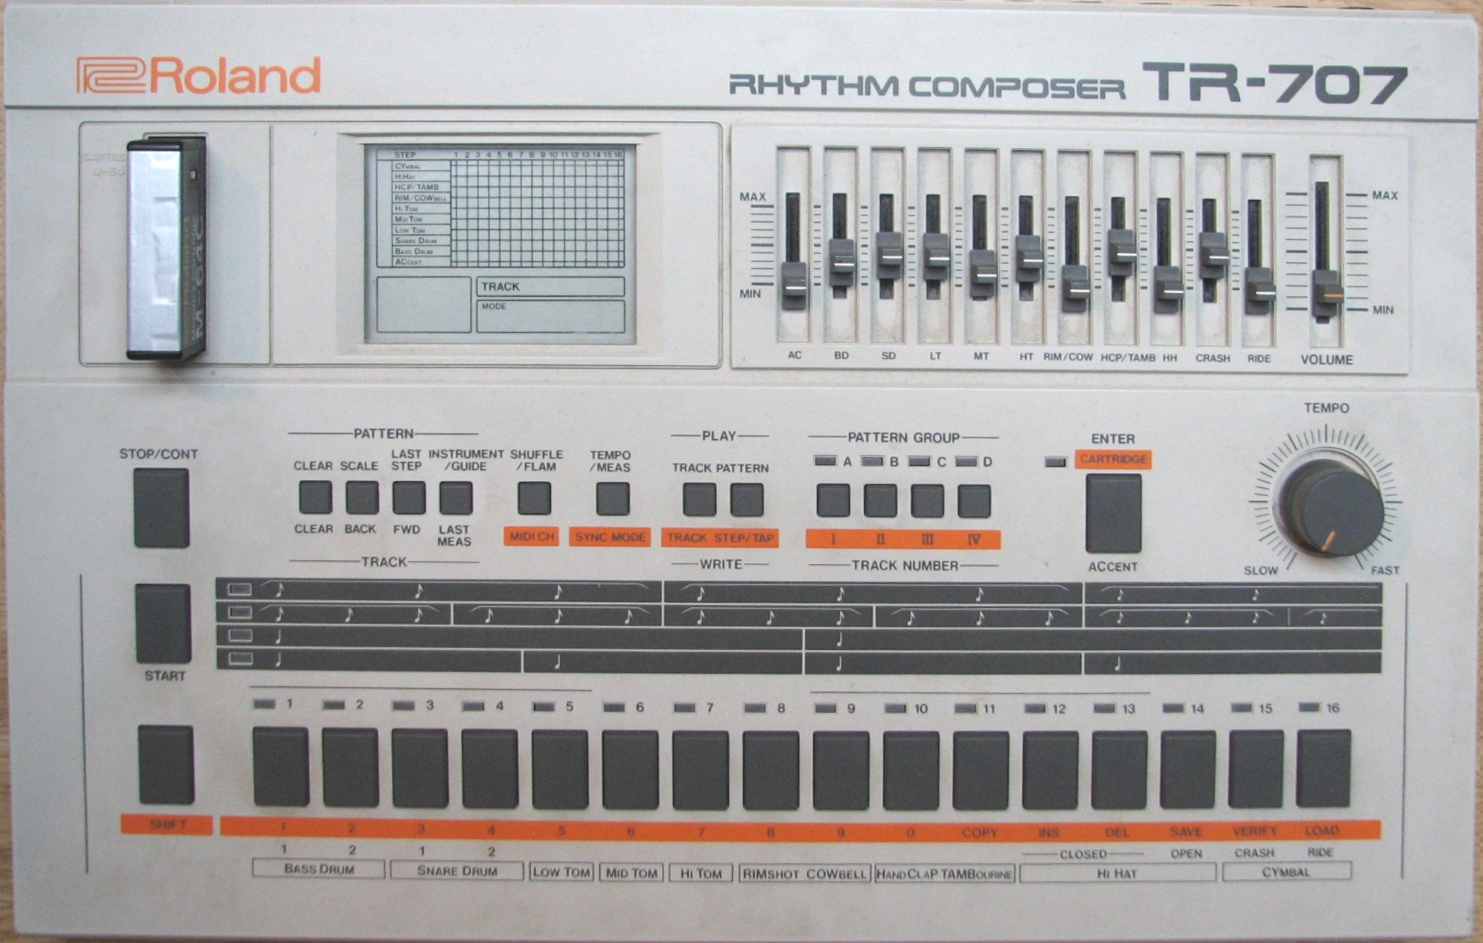
\includegraphics[width=5in]{Henry Thesis/Images/Roland_TR-707_edit}
\caption{Roland TR-707 Front Panel}
\label{fig:TR707}
\end{centering} 
\end{figure}

The percussion on ``Krakpot'' comes from the Roland TR-707, a piece of studio equipment that was also adopted by house and techno producers. The TR-707 plays digital samples, which makes it more static than Roland's earlier analog synthesis-based drum machines like the TR-909 and TR-808. The bottom row of the TR-707 panel, shown in Figure \ref{fig:TR707} contains 16 buttons for inputting and programming drum patterns.\footnote{\cite{speculosDrumMachineRoland2008}} In the top right corner are 12 volume sliders, 11 for the various drum sounds and one for the master volume which Hawtin uses in combination with external effects to bring the drums to life.

With careful listening, during the first four minutes one can hear a reverb tail build up and fade away around the bass drum. The effect repeats with some regularity giving subtle movement to the beginning of the recording as other percussive elements do not begin to appear until 4:22. A transcription of the rhythm is shown in Figure \ref{fig:krakpot_drums}. The hi-hats and cowbell fade in with great restraint and the short hi-hat pattern gains movement from gradual phase modulation, an effect caused by the audio signal mixing with an out-of-sync copy of itself, similar to Steve Reich's tape phasing music.\footnote{\cite{huizengaFiftyYearsSteve2015}} The phasing lends a simulated ``live'' feeling to the groove with its continuous sense of movement. A syncopated clap rhythm begins to fade in at 5:25 as delay changes the perception of percussion density, building rhythmic echoes off the clap and cowbell. Only one full drum pattern is used through the track, which stays in form with the TB-303. 

\begin{figure}[htbp]
\begin{centering} 

\includegraphics[width=6in]{Henry Thesis/Images/Krakpot_Drums2}
\caption{Drum Transcription of ``Krakpot''}
\label{fig:krakpot_drums}
\end{centering} 
\end{figure}

The gradual entrance of each percussive element keeps ``Krakpot'' from growing tired. When the crash cymbal enters 7:03, Hawtin fades it out a short 8 bars later, leaving it as an overpowering burst of energy that marks the peak moment of the piece. Percussion is drawn out of the mix from 7:27 onward, and disappears entirely by 8:22. The bass drum drops out at 8:27 and Hawtin plays the TB-303 through a short dramatic solo where the filter pulls up rumbling bass resonances to a crescendo at 9:12 before easing off. Hawtin brings the bass drum back for the final wind down at 9:27 and ``Krakpot'' ends with the bass drum, without reverb or additional percussion.

As a full piece, ``Krakpot'' has one energetic arc, building up energy towards the seven minute mark and fading out gradually to the end. This single path works well for the constant bass rhythm, which is made more effective without interruption. However minimalism does not need to keep itself to a single arc of energy, and can explore building energy and tension over combinations of peaks and valleys of energy.  

\newpage
\section{Structure and Tension: ``Lost In Space'' by Subsonic}
\label{sec:lostinspace}

\subsection{Background}

Dynamic in structure and instrumentation are in focus through analysis of ``Lost in Space'' by Subsonic. ``Lost In Space'' is a long trip, at around 14 minutes, and rockets along at 150 beats per minute. Little information is available on the producer. Writing credits are attributed to Ben Phillips, and Subsonic had two releases on the UK label Direct Current, 1995's \emph{Lost In Space} and the follow up \emph{Subsonic EsP} in 1996.\footnote{\cite{SubsonicSubsonicEsP}, \cite{subsonicLostInSpace1995}} (Direct Current itself closed after five releases in 1997.)\footnote{\cite{DirectCurrent}} What we are left with is a shining example of the UK acid-techno sound in the mid-1990s. Put under the microscope here are the methods employed by Subsonic to manage energy in ``Lost in Space''-- building up layers of sound, muting instruments, and creating sonic space.

\subsection{Instrumentation and Patterns}

``Lost In Space'' counts eight different instruments in its arrangement, which are listed on the left column of Figure \ref{fig:lostinspace}. An additional robotic ``Lost In Space'' vocal sample repeats at semi-regular intervals. ``Lost In Space'' is based around a partial B$\flat$ Phrygian scale, with only F, G$\flat$, A$\flat$, B$\flat$ and C$\flat$ from the scale. B$\flat$ holds the melodic center in all three melodies transcribed in Figure \ref{fig:lostinspace} while generous half step movement gives an aggressive edge to the music.

\begin{figure}
\begin{centering} 

\includegraphics[width=6in]{Henry Thesis/Images/Lost_in_Space_3}
\caption{Transcription of ``Lost In Space''}
\label{fig:lostinspace}
\end{centering} 
\end{figure}

\subsubsection{TB-303}

The Roland TB-303 is an expected choice for an acid track and on ``Lost In Space'' it is the most prominent synthesizer. Contrasting the use of the TB-303 in ``Krakpot,'' here the synth is subject to extreme distortion that brings out a more aggressive timbre. The additional overtones brought out by distortion give a stronger impression of a second voice made from the snarling resonance. Accents on the TB-303 keep the sound changing by increasing the amount of distortion for brief moments as specific notes are pushed louder. A short delay is mixed with the TB-303 and provide spatial dimension to the overdriven bass line.

The TB-303 pattern is the primary source of musical intrigue for ``Lost In Space,'' and has the most complex melodic line. Transcribed in Figure \ref{fig:lostinspace}, two accented eighth notes on B$\flat$ start the pattern with a burst of energy, followed by a half step slide from F that syncopates the second half of the pattern. The accented and syncopated notes that follow rise from B$\flat$ to C$\flat$ and up to A$\flat$. The two octave leaps down from B$\flat$ are almost inaudible in the mix, because of this they give space to the higher pitches. At the end of the bar is a burst of three sixteenth notes on G$\flat$, that functions as a pickup to the start of the loop.

\subsubsection{Sub Bass}

In a the same frequency range as the TB-303 is a synthesizer I am calling the ``Sub Bass.'' The sound is a chorused saw wave, treated with spacious reverb and delay. It adds a murky bass rumble beneath the TB-303 and plays a pattern of B$\flat$ with upper and lower neighbor notes, a motif consistent with the other melodic elements.

\subsubsection{Ambient Pad}

An eerie, undulating, sine-wave-based string sound is the last melodic component, bringing a moody, dissonant atmosphere to quieter moments of the piece. The ``ambient pad'' also uses the B$\flat$ and C$\flat$ theme, over a four-bar loop. No fundamental harmony is changed by the pad, but it creates the closest thing to a tonal progression, alternating emphasis from B$\flat$ to C$\flat$.

\subsubsection{Roland TR-909}

\begin{figure}
\begin{centering} 
\includegraphics[width=\columnwidth]{Henry Thesis/Images/Roland_TR-909}
\caption{Roland TR-909 Front Panel}
\label{fig:TR909}
\end{centering} 
\end{figure}

The bulk of the percussion on ``Lost In Space'' comes from the Roland TR-909. The follow up to Roland's TR-808, the TR-909 was released in 1984, and is another machine synonymous with the sound of house and techno. The TR-909 features a blend of synthesized and sampled percussion, allowing fine timbral adjustments and more ``realistic'' drum sounds compared to the TR-808.\footnote{\cite{annissInstrumentalInstruments9092016}} The controls of the TR-909 are shown in Figure \ref{fig:TR909}, and are similar to the TR-707 and TR-808, with a row of 16 buttons for programming patterns.\footnote{\cite{clusternoteRolandTR9092011}} Each instrument has dedicated knobs for controlling volume and parameters like attack, decay and pitch. These controls make performing dynamic changes easier on the TR-909 than on other drum machines, an aspect of the instrument used by artists like Jeff Mills in DJ sets and improvised performances.\footnote{\cite{millsJeffMillsExhibitionist}} On ``Lost In Space'' the TR-909 is responsible for the clean and consistent punch of the bass drum that pins down the quarter-note pulse. The TR-909 clap plays on beats two and four, and the open hi-hat fills the offbeat gaps. These rhythms are all notated on Figure \ref{fig:lostinspace}, page \pageref{fig:lostinspace}.

Additional percussion comes in the form of a small burst of white noise, similar in timbre to a shaker, which pops up at the end of each bar. A delay on the noise shaker has enough feedback to sustain the signal through the bar and filter sweeps on the noise signal can be heard at moments like 11:45--11:51. A second hi-hat, with a distinct sound that lacks the lower frequency weight of the TR-909 hi-hat, plays a similar pattern to the TR-909 pattern with a sixteenth-note crescendo at the end of the bar. 

\subsection{Structure}

The structure of ``Lost In Space'' is charted in Figure \ref{fig:structure}. The chart is based on how one might view the structure in a Digital Audio Workstation (DAW) such as Ableton Live or Steinberg Cubase. The diagram shows where patterns and their corresponding instruments enter and exit the mix. Each instrument has a color-coded track, and colored blocks corresponds to where an instrument is active. Half-length vertical lines in the blocks represent pattern length, which is one bar in most cases, except for the four-bar ambient pad. The chart is paired with a volume waveform to help visualize changes in dynamics.\footnote{The waveform was rendered using Audacity and converted to a vector image.} The waveform represents amplitude over time, on a logarithmic scale of -1 to 1, with zero representing silence.

Certain sections of the structure are more subjective than others, like at mm. 417 when the ambient pad is pulled back in the mix such that it is masked by other elements and becomes almost inaudible. My chart may not be exact as to how other listeners may hear elements coming in and out of the mix, but serves the purpose of providing an overview of the structural changes. Volume and filter automation are not included on the diagram, as it is difficult to convey on a chart of this scale. Filter changes are also not the primary object of this analysis; however both volume and filter automation are significant and will be discussed as necessary.

\begin{figure}
    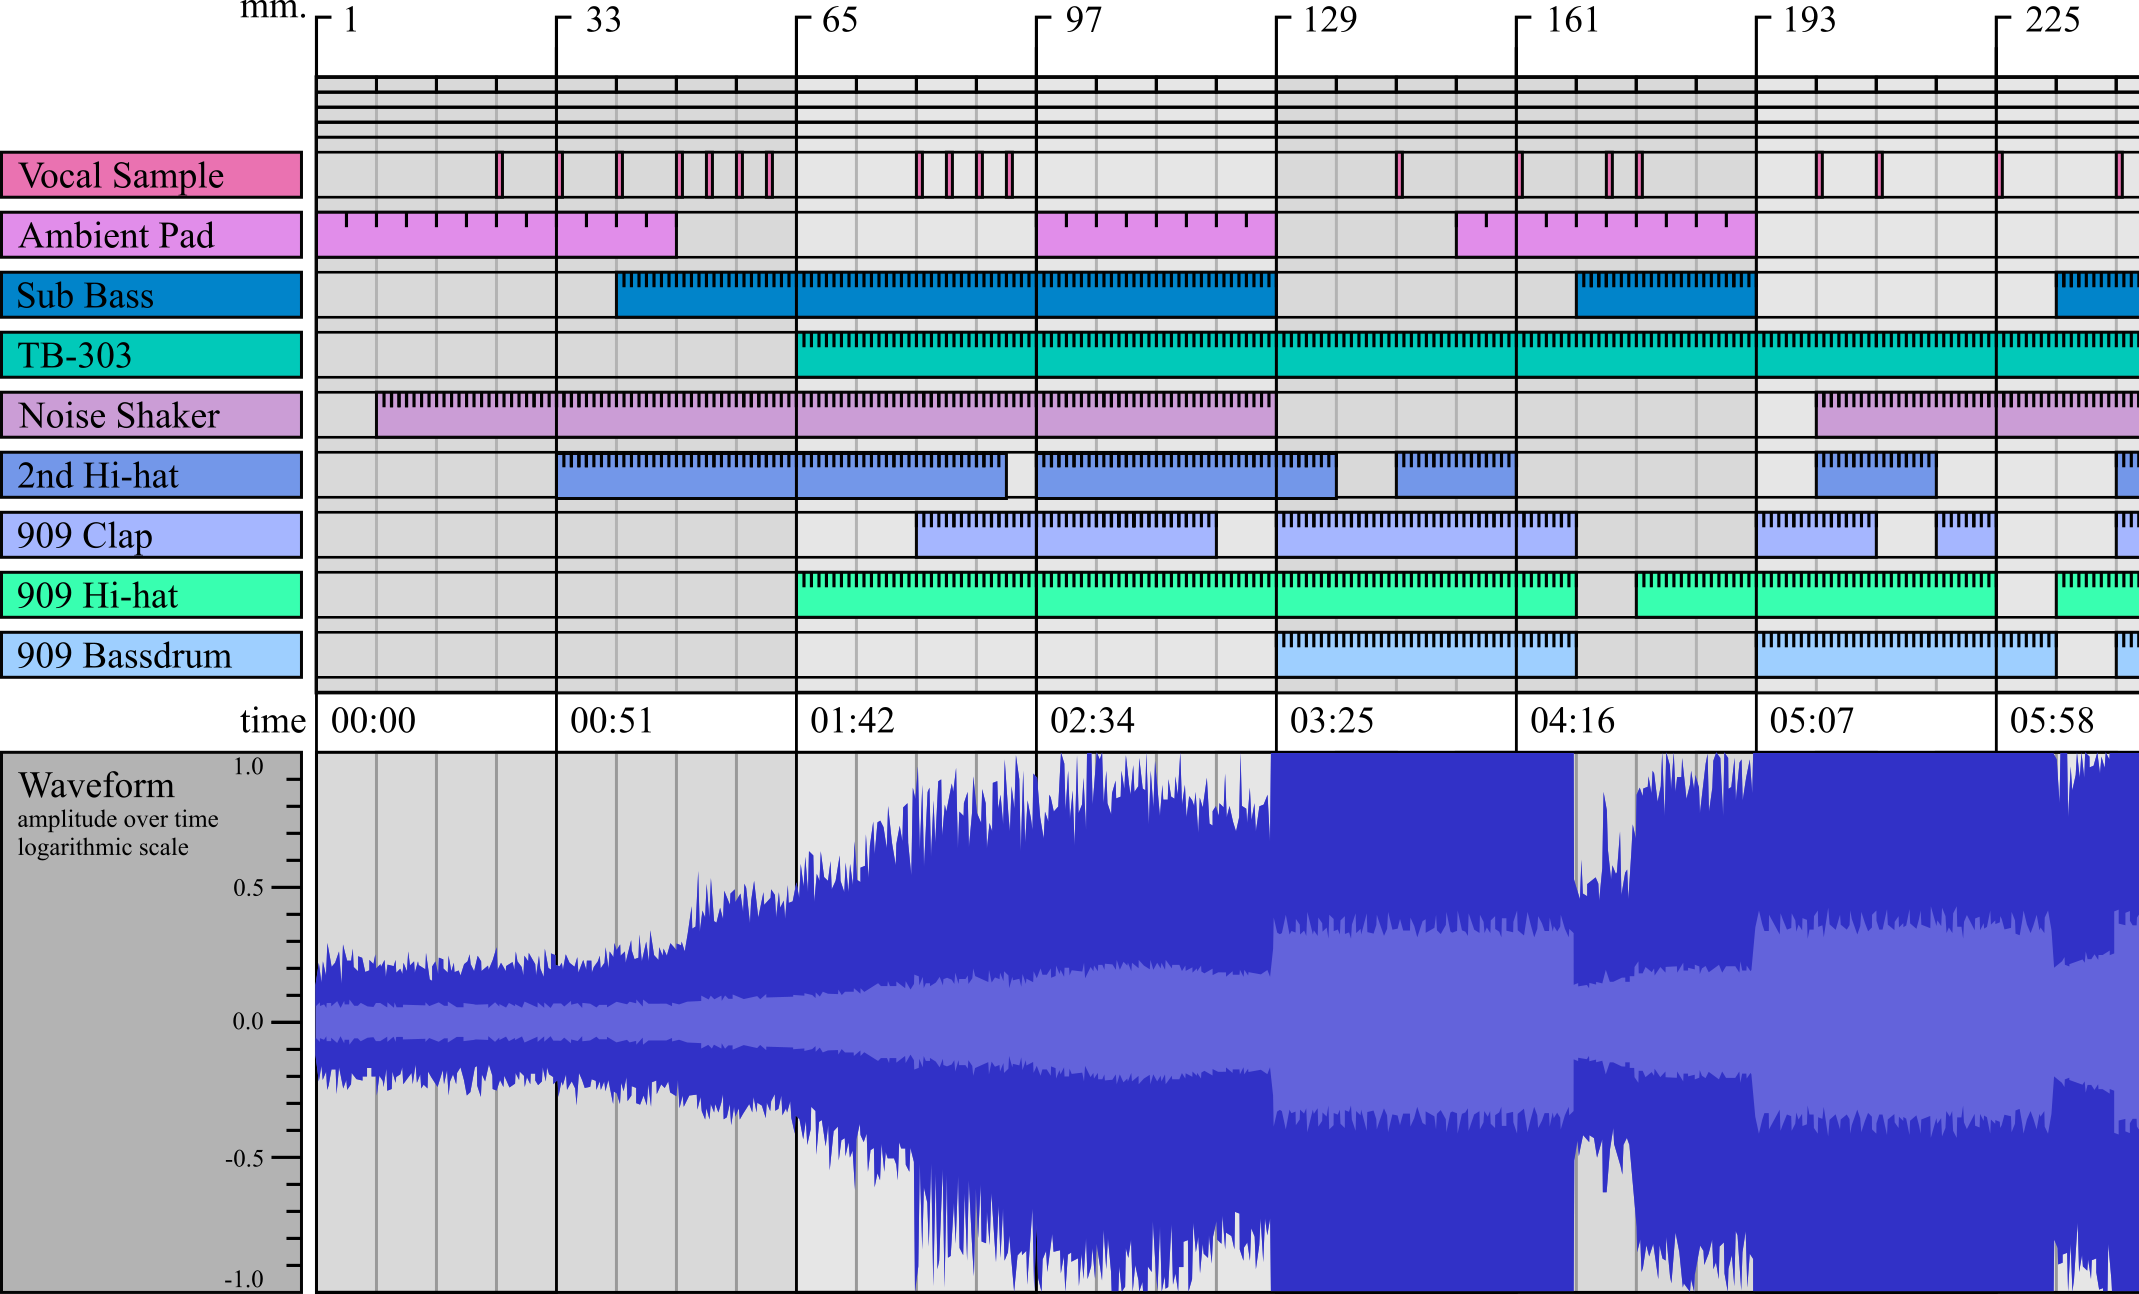
\includegraphics[width=\columnwidth]{Henry Thesis/Images/STRUCTURE_FINAL_L}
    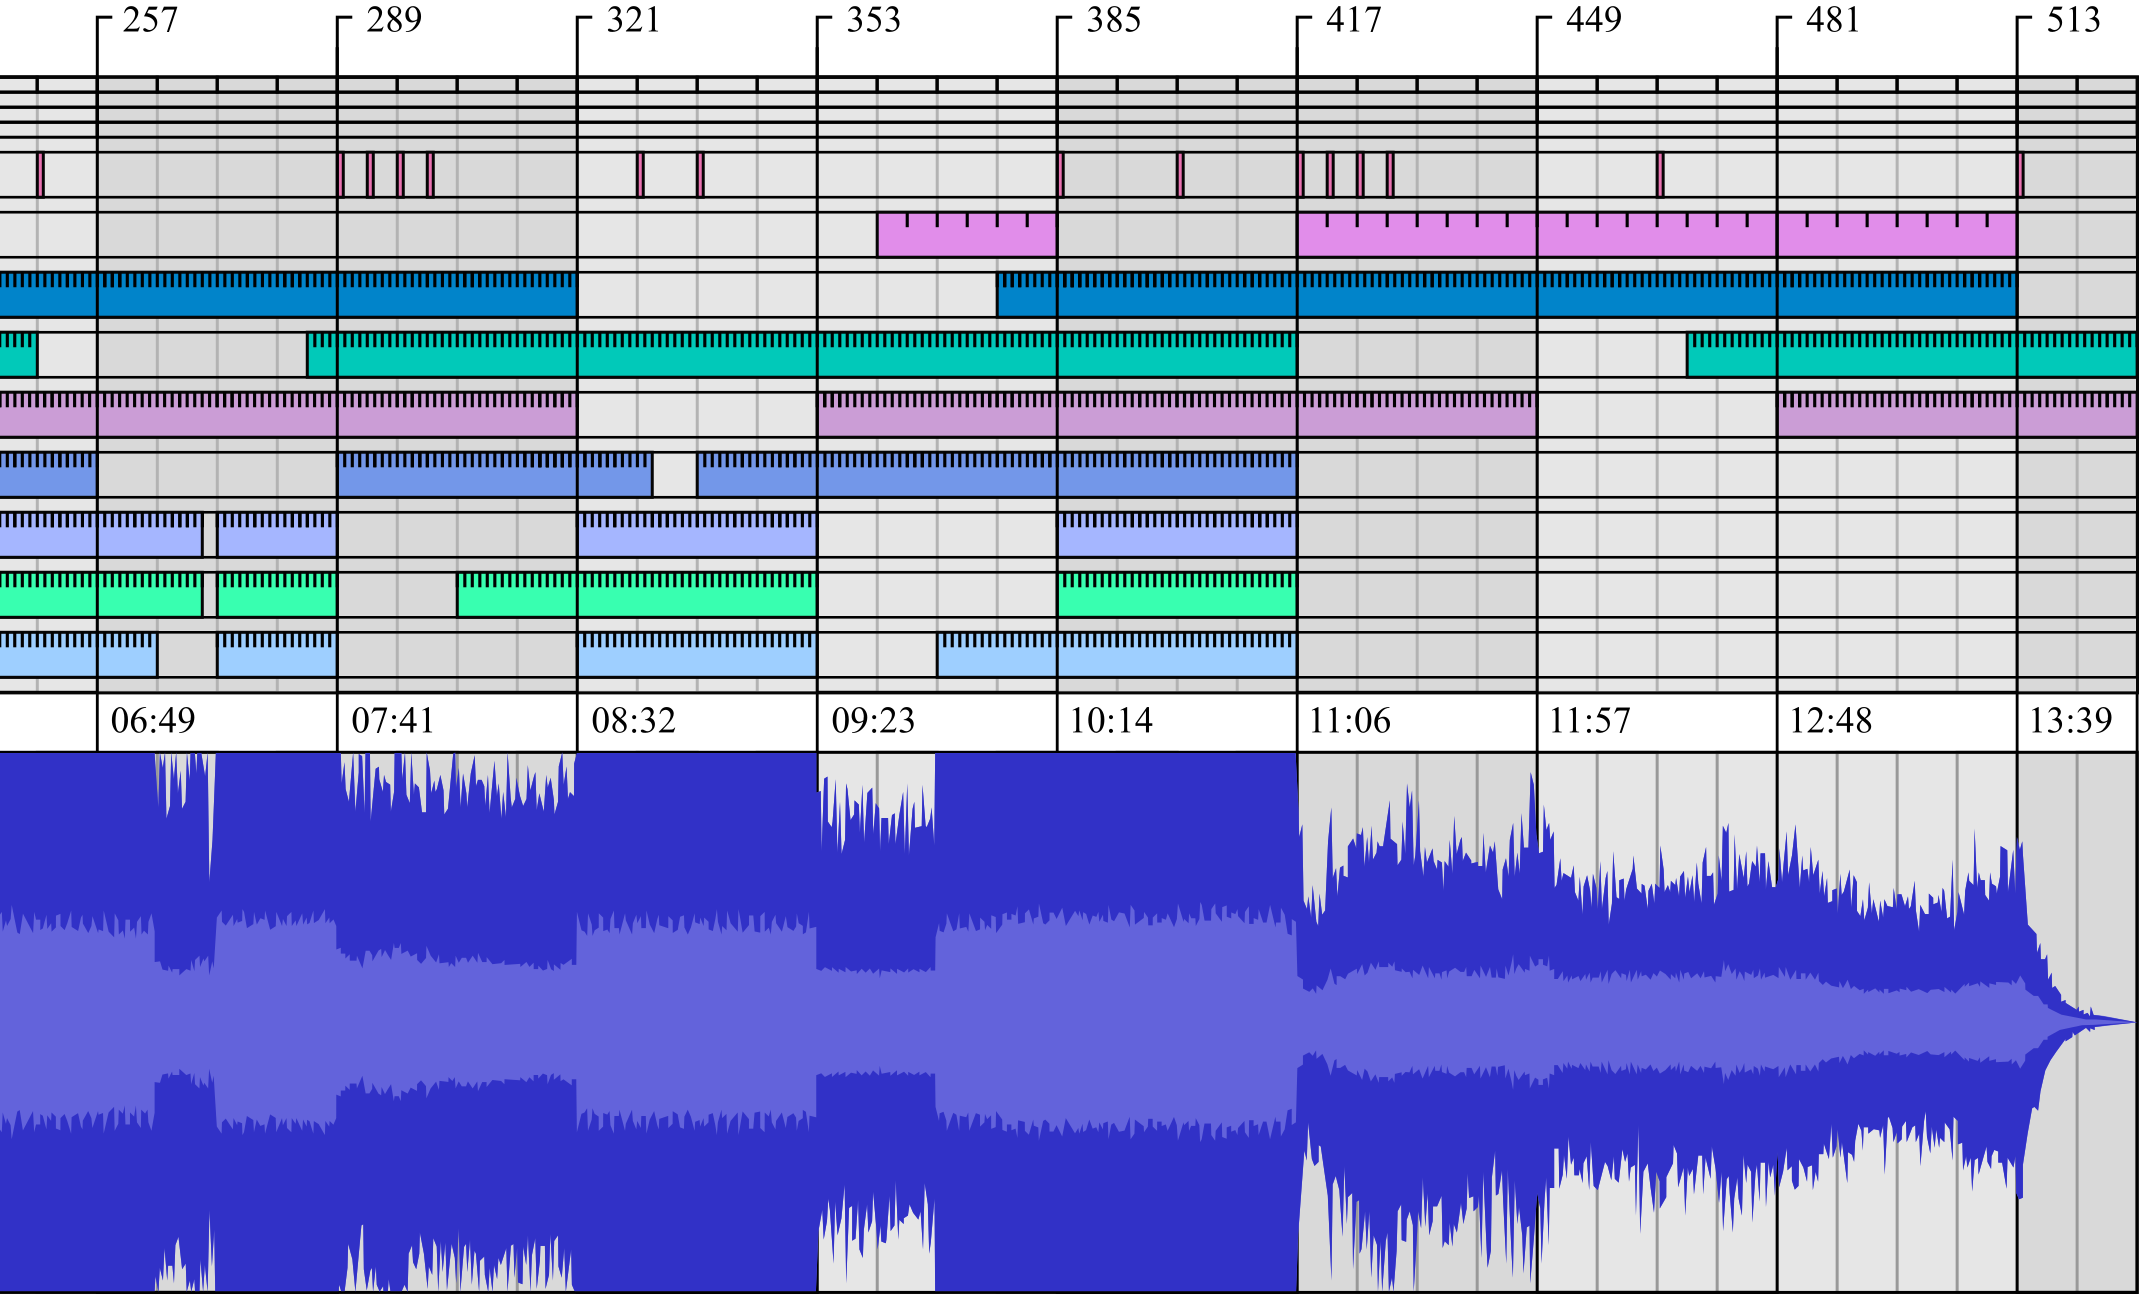
\includegraphics[width=\columnwidth]{Henry Thesis/Images/STRUCTURE_FINAL_R}
    \caption{Structural Analysis of ``Lost In Space'' with Volume Waveform}
    \label{fig:structure}
\end{figure}

\subsubsection{Building and Releasing Tension}
``Lost In Space'' builds energy slowly as instruments are introduced to the mix with a cautious pace. Starting with the ambient pad, the shaker fades in first, and the secondary hi-hat follows at mm. 33 (00:51) introducing a rhythmic pulse. The sub bass becomes audible four bars later and the half-step melody sets the listener on edge waiting for some kind of cadence. The ``lost in space'' vocal sample begins repeating once every eight bars and the rate doubles to once every four at mm. 49 (1:16), prior to the TB-303 and TR-909 hi-hat fading in at mm. 65 (1:42).

When the ambient pad cuts out at mm. 49, a consistent pattern of 16-bar change is established. The TB-303 and TR-909 hi-hat enter at mm. 65 and the TR-909 clap has a sudden fade in at mm. 81. The secondary hi-hat disappears for four bars at mm. 93 and when it returns with refreshed rhythmic energy at mm. 97 it marks the second climb of the intro section. The ambient pad returns to the mix and all other elements at full volume and the resonance of the TB-303 climbs higher. When the clap drops out at mm. 121 (3:12) everything has built towards the entrance of the bass drum at mm. 129---better known as the beat drop.

After three minutes of rising energy the bass drum finally enters. Combined with the sudden removal of the sub bass, the bass drum shifts the energy of ``Lost In Space'' significantly. The force of 150bpm comes to the forefront, crisp and clear compared to hi-hats in the the opening section. Mirroring the frenetic pace, the rate of change quickens to every eight bars between mm. 129 and 169. The sudden disappearance of the sub bass lets the TB-303 move to the forefront as the primary bass synth. The air between notes in the TB-303 pattern is also pronounced against the simpler musical backdrop, further amplifying the rhythmic pulse. 

A 24-bar breakdown starts at mm. 169, dipping the energy briefly before another bass drum section starts at mm. 193. The TB-303 envelope modulation shortens abruptly during mm. 201 (5:20), and the accented notes become more pronounced in the following bar. At mm. 241 (6:24) the sub bass starts to compete with the three other low-frequency instruments, having avoided overlap with the bass drum until now. The TB-303 loses the fight and fades out eight bars later letting the sub bass pulls to the front of the mix. The bass drum is present in the mix for progressively shorter lengths of time, from 40 bars, to 24, to 16 between mm. 193 and mm. 289 (5:07 - 7:41.) These shortened phrases are like moments of indecision before the bass drum cuts out for the breakdown and build at mm. 289. 

Beginning at mm. 257 (6:49) the reverb on the sub bass increases and the sound shifts into a different role. The dense reverb makes it hard to tell what exactly happened, my hypothesis is that unprocessed synth signal was faded out of the mix, and the reverb was left. Measure 277 (7:21) points to this change when the sub bass riff is transposed up a second octave and the dry signal fades in briefly. The TB-303 rushes back into the mix at mm. 289, reclaiming its position as the main bass synthesizer. At mm. 321 ``Lost In Space'' mirrors the phrase at mm. 129, with emphasis on the sudden disappearance of the sub bass in the previous phrase, and the same active instruments.

Measure 353 is the last intermediate breakdown started when the bulk of the TR-909 percussion drops out for 16 bars. The bass drum is brought back with the ambient pad to build toward the final crescendo at mm. 385. Almost every part of the mix is active at mm. 385, creating a dense sonic moment that dissipates into an ambient breakdown at mm. 417.

The ambient section gradually tapers off in 32-bar waves. The sub bass returns in washes of reverb, and fights for room in the mix with the ambient pad. The TB-303 fades in for another build of energy, but fades out at mm. 469, staying low in the mix. The last instance of the vocal sample occurs at mm. 513, and the TB-303 and noise shaker fade to silence. This brings ``Lost In Space'' to a close, having guided the listener over mountains of sound, into small valleys of relative calm, and up trails of anticipation, before drifting away in an ocean of ambience.


\newpage
\section{Change and Confusion: ``Phylyps Trak'' by Basic Channel}
\label{sec:phylyps}

\subsection{Background}

Where the previous two pieces fit within the techno and acid house frameworks, ``Phylyps Trak'' is a defining piece of early dub-techno by Basic Channel, measuring in at 144 beats per minute and just under ten minutes long.\footnote{\cite{basicchannelPhylypsTrak1993}}  While synth resonance is one of the dominant features of acid, dub-techno gravitates towards the rhythms of syncopated chords paired with varying amounts of delay and reverb. The structure may be more difficult to discern with delays prolonging and emphasizing offbeat rhythms, and gradual changes obscuring lines between phrases and layers.

\subsection{Instrumentation and Patterns}

In ``Phylyps Trak'' Basic Channel mixes eight different loops into a single sonic fabric, gluing together the timbre and rhythm with saturation and spatial effects. Five pitched loops cycle in and out, each with specific rhythmic and timbral characteristics. These loops combined create a dynamic pattern that is manipulated throughout the recording. Centered around G minor, ``Phylyps Trak'' emphasizes perfect fifth intervals and minor triads. The fundamental frequencies that clarify the pitch of a notes, are cut out by a high pass filter on many loops. This puts emphasis on the noisier frequencies, which define the timbre more than the tonality of each chord. As rhythmic interaction is one of the key parts of this piece, my transcription in Figure \ref{fig:phylyprytm} on \pageref{fig:phylyprytm} is a rhythmic reduction meant to clarify how the rhythms interact.

\begin{figure}
\begin{centering} 

\includegraphics[width=6in]{Henry Thesis/Images/PhylypsTrakNotation4}
\caption{Rhythmic Transcription of ``Phylyps Trak''}
\label{fig:phylyprytm}
\end{centering} 
\end{figure}

The bass loop on Figure \ref{fig:phylyprytm} has the timbre of a throaty growl and sounds to contain more harmonic content than a single note. My guess, made by inspecting the sound on a frequency analyzer, is that the sound is created by playing two notes in harmony, one low enough that it effects the primary bass note as a low frequency oscillator. The bass also has an unusual movement across the stereo field, something avoided when making music meant to be cut to vinyl, as it can cause a needle to jump out of the groove.\footnote{\cite{hooseTurningTablesEngineering2018}, 9.}

The first two stabs of the primary chord loop shown in Figure \ref{fig:phylyprytm} play a dotted-quarter rhythm in the first bar, but on the second bar are syncopated off the downbeat. The stabs sound on the second 16th note of the beat, imitating the syncopation in the bass loop. Only the first chord lands on the downbeat. The secondary chord loop fills in gaps left by the primary loop, and adds emphasis to the last chord of the first bar. The tertiary loop fits in with a dotted-eighth burst that that mirrors the rhythmic transformation of the primary loop on the second bar. The dotted-eighth chord loop is the highest-pitched loop, and plays a continuous dotted-eighth rhythmic pattern that restarts on the last beat of the second bar. By not restarting on beat one, the dotted-eighth loop blurs an otherwise clear phrase length and downbeat.

The familiar Roland TR-909 is the percussive engine on ``Phylyps Trak,'' and Von Oswald and Ernestus only use the bass drum, clap and hi-hat from the machine. While the bass drum remains dry and tight with the clap, both are contrasted with the airy, open hi-hat. Despite the simple pattern, it remains driving throughout, as the reverb keeps the hi-hat live and engaging.

\subsection{Structural Disorientation}

In ``Phylyps Trak,'' a seamless thematic progression occurs in mix of active chord loops, accomplished through subtle changes in mix and unannounced changes in phrase that can slip past the listener. Based on recording practices in early 90s techno, the structure of ``Phylyps Trak'' was probably created live. The gradual fade-in of each loop and slow phrasing feels unlike the clear 48 bar phrases in ``Lost In Space.'' The recording is also a contemporary of ``Krakpot,'' and it is easy to infer that the same production technique of ``jam for 20 minutes or half an hour, afterwards do some editing'' as Richie Hawtin put it, would be used here.\footnote{\cite{burnsRichieHawtinLecture2013}} It becomes even more likely taking into account the Detroit connections that Basic Channel had made, through Juan Atkins, Carl Craig, and others who used the live technique Hawtin drew upon. 

``Phylyps Trak'' starts with an abrupt, noisy fade in, like that of a skipping record. The fade in, combined with syncopated rhythmic emphasis in the loop, obscures the listener's perception of the first beat. For instance, I hear beat one as the second sixteenth-note of the second bar, on the chord stab. This rhythmic deception holds until the bass drum bursts in at 0:39 and the pulse reveals the beat to be an unexpected sixteenth-note earlier. The pattern has changed in a dramatic but subtle way by altering the perceived pulse. Through repetition, the groove sounds to realigns with the bass drum, however nothing has changed. The open hi-hat fades in next and further cements the four-on-the-floor rhythm.

Twenty four bars after the bass drum, the second chord loop joins the mix, and in doing so, maintains a consistent rate of entrance. However when the bass drum suddenly cuts out after 17 bars, it breaks the eight-bar-based phrase structure and the regular pace is thrown into temporary disarray. Basic Channel continues play with and ignore concepts of even pacing for the remainder of the track.

Returning from the brief breakdown without the bass drum, all three percussive elements come back into the mix. The bass drum stays put for the rest of the track and the hi-hat and clap remain undisturbed for the next three minutes, so changes come from the chord loops. At 2:48, the primary chord loop is supplanted by the dotted-eighth loop fading in. At 4:00, or 43 bars later, the chords exchange again, with the tertiary loop taking the place of the primary loop. The gradual mixing also makes points of transition hard to pinpoint and serves to blur any separation of phrase, making the track seem less prone to change than it really is.

Considering the short and syncopated loops in ``Phylyps Trak'' it may be unclear if what I defined as beat one in Figure \ref{fig:phylyprytm} is what Von Oswald and Ernestus understood beat one to be in sequencing. It is possible that the downbeat is the three of either bar, taking into consideration how the track fades in, and moments where musical elements drop out mid-bar. In moments like 4:49 for example, when the dotted-eighth loop is cut from the mix, it seems to be removed at beat three of the bar, and appears again exactly eight bars later on beat three again. Despite this grey area, I am confident about where I placed beat one in Figure \ref{fig:phylyprytm}. The accented primary chord loop and bass note on that beat is one of few synchronous rhythmic points in ``Phylyps Trak'' and where the bass drum enters at 0:39 is on this beat as well. If it was not written as the first beat, it certainly sounds like it is.

A sudden change in ``Phylyps Trak'' happens at 5:25 when the instrumentation switches to the secondary chord loop playing against the percussion and bass. The primary chord loop returns to the mix gradually alongside the open hi-hat. At 6:58 the upper percussion drops out of the mix and re-appears roughly a minute later. This time the percussion is accompanied by a different pair of chord loops, the dotted-eighth and tertiary chord loops, as the primary and secondary loops fade out. Ending on loops that are different from the ones in the opening creates a thematic progression in ``Phylyps Trak.'' The progression is gradual enough that sudden small changes are amplified in impact and slow fades can be missed without close listening, re-applying concepts of ``music as a gradual process.''

\section{Conclusion}

A clear and narrow vision of techno appears among the pieces analyzed, which can be drawn upon as a model for composition. ``Krakpot,'' ``Lost In Space,'' and ``Phylyps Trak'' all rely on a quarter note kick drum in 4/4 time like many techno tracks. Hi-hats fill the off beats, and a clap or snare plays on beats 2 and 4---a drum pattern one can also find in disco and house.\footnote{\cite{maloneyHouseMusicWas2018}, 234.}

A syncopated bass riff fills in the space between the quarter notes on all three tracks, and all are over 10 minute long with no contrasting B phrase. Instead, musical elements are brought in and out with different timings and combinations to sustain interest. Most patterns last only one bar on these recordings, with four- and two-bar loops occurring less often. A limited palette of harmonic gestures is also preferred: simple triads for ``Phylyps Trak,'' neighbor notes and octave leaps for ``Krakpot'' and ``Lost In Space.''

Achieving a distinct sonic character through production is also essential. Without effects, the recordings would lack a compelling sense of movement. Delay and echo create interweaving melodic lines and add harmonic and rhythmic complexity to a pattern. Reverb and filter movement alters spatial and timbral character---moving sounds through dimensions and sonic placement. Signal processing also gives individual flair to common drum machine and synth sounds from the TR-909 and TB-303. In each recording these instruments are processed in different ways, adapted to fit the context of the track at hand. The recording may start with the same basic sound, but the end result is unique.

The ``minimalist'' aesthetic the pieces reflect comes in several forms. The rhythms and melodies are often simple, consistent, short phrases with limited pitch content. These simple patterns combine with other patterns and loops, a mix of raw musical materials that form something more complex through repetition. The slow permutations and sonic modulations give movement and growth to these patterns over time, helping limit uninteresting ``perfect'' repetition. These features---sonic palettes, effect modulation, and extended structures grown from short patterns are key influences for my own compositions.

\chapter{\emph{Nipper's Trip}}

\begin{figure}
\begin{centering} 
\includegraphics[width=6in]{Henry Thesis/Images/ALBUM_ART}
\caption{\emph{Nipper Reigns Over a New Era of Consciousness} (2021) by Laurie Duffy}
\label{fig:albumart}
\end{centering} 
\end{figure}

The limitations of vinyl records and the hypnotic sounds of acid techno are the largest inspirations I drew upon for my compositions ``Heaven {\&} Earth'' and ``Escitalopram.'' Vinyl twelve-inches often follow the A-side and B-side binary in dance music. The A-side is often the more club-focused track, which in this case is the corrosive techno-trance piece ``Escitalopram.'' Since the A-side is meant to sell the record, the B-side can be more experimental, and ``Heaven {\&} Earth'' is freed to explore sonic dimensions that might not work in a DJ set. Both tracks carry the calling card sounds of acid techno, the TR-909 and TB-303. In lieu of a real Roland TB-303, I used a clone called the Cyclone Analogic TT-303, and without an original analog TR-909, digital samples sufficed. Harmonic and melodic content is secondary to changes in timbre and mix on both tracks, a compositional approach inspired by the music I analyzed beforehand. Discussing the pieces and my creative process makes the most sense when done in the order in which I composed them, beginning with ``Heaven {\&} Earth.''

\section{``Heaven {\&} Earth''}

\subsection{Inspiration}

``Heaven {\&} Earth'' is based on the organic and fluid structures of minimal techno: the gradual progressions on ``Phylyps Trak'' and "Krakpot," and the cavernous chambers of sound in the work of artists like Monolake and DeepChord. Written at 133.3 beats per minute, one bar is 1.8-seconds long, which matches one revolution of a record at 33.3 rpm. This allows a mastering engineer to cut a record with a locked groove that loops in time.\footnote{\cite{AardvarkRecordMastering}} This feature is unique to vinyl as a medium, and was inspired by the locked grooves on records by Jeff Mills and the Los Angeles based Exist Dance label.\footnote{\cite{upaboveTryingTo1993}} ``Heaven {\&} Earth'' also nears the longest duration of audio---around 18 minutes---that can fit on a record before the mastering engineer has to cut the disc at an incredibly quiet volume.\footnote{\cite{hooseTurningTablesEngineering2018}, 4.} The short TT-303 bass line keeps to the same pattern for the whole duration, mirroring the constant repetition in other minimal pieces. Melodic lines are written in a vague F Phrygian, drawing on the use of half steps in works like ``Lost in Space.'' The name comes from the vocal sample, which unedited is ``Before heaven and earth, there was something nebulous.'' The sample is an otherworldly, psychedelic sound clip borrowed from Dr. Timothy Leary's 1967 album \emph{Turn On, Tune In, Drop Out} that gave the piece focus and direction.\footnote{\cite{learyTurnOn1967}}

\subsection{Form and Process}

To create a natural progression of energy, the form was developed from a live take on the TT-303 synthesizer, with only a bass drum accompanying. With no structural guidelines, I made filter changes and forays into new timbres as I felt they were needed. Recording it live let me pace the filter movement to my attention span, and freed me from the rigid grid of four-, eight- and sixteen-bar cycles.

After recording the TT-303, I continued to build new layers in similar takes. Percussion followed in subsequent takes---clap, hi-hat, bongos, and the ride cymbal---each with unique modulations and undulations. Most percussive layers were recorded with live application of reverb and delay effects as well.  Adding the percussion solidified the energetic path of the piece, and it allowed me to replace the bass with an alternate take. I found my the original take on the TT-303 had become too flat when put alongside the drums. Thanks to this layer by layer approach, I was able to mix the track as I recorded each part, and improvise with my past self. The bongos move through distortion as an out-of-phase, eighth-note delay slowly alters the rhythmic density. In contrast the hi-hats are sent through delay and reverb in sudden bursts in quiet moments like at 12:01.

Building layers of takes was my way to adapt the live recording techniques of Plastikman and Basic Channel to my own recording process. Due to technological constraints, I only fed a stereo channel out of my mixer and without recording multiple takes I would be unable to apply EQ and compression in post-production. 

With the rhythm section recorded, I moved on to the vocal sample. The phrases ``before heaven and earth'' and ``something nebulous'' are panned left and right in a staggered rhythm. The sample is truncated and edited through the track as well, altering rhythmic placement. The variations are akin to those of minimalist composers who generated rhythms and interest with spoken recordings looped into rhythmic phrases.

The chord that echoes through the piece is shaped by adjustments to the filter cut-off and envelope release which lets it fit in more contexts than an unchanging sound might be able to do. The flute patch that appears at 4:19 was a sudden improvisation and brings a longer melodic contour to the piece. The flute was recorded with percussion muted, so my playing drifts around the pulse a bit, which helps to offset the strict drum machine rhythms. The flute also uses the same delay with which the TT-303, hi-hats and chord are processed. The delay was programmed on an Alesis Quadraverb as a dotted-eighth note ``ping-pong'' delay. A 10 cent de-tune that adds a wobble and long reverb are also part of the effect program, adding a greater degree of movement and modulation. By mixing different instruments into one delay, a coherent sense of space and dimension is added to the piece. 

\section{``Escitalopram''}

\subsection{Inspiration}

``Escitalopram'' belongs in the same realm as the blistering acid techno of ``Lost In Space'' and much less the ambient dub-techno that ``Heaven {\&} Earth'' draws on. Early sketches of ``Heaven {\&} Earth'' were set at 150bpm, but the piece developed differently and I wanted to incorporate that exhilarating tempo into my work, so I revisited the tempo for the second track. Rather than gradual adjustments, sudden changes in instrumentation sustain interest, with occasional one-bar track mutes and edits. Part of the sudden nature of the pieces comes from the speed at which I wrote the track. I began ``Escitalopram'' on a Friday morning, and by Saturday afternoon I had a final structure in place. The title is a play on the prominence of substances like ecstasy, LSD, and weed, among others, that permeate rave culture and track naming conventions. Escitalopram is the scientific name of the serotonin-fuelling drug I take everyday, otherwise known as the anti-depressant Lexapro.\footnote{In particular, I found the track ``Prozac'' by Geezer and realized anti-depressants are good track titles-- \cite{geezerProzac1996}} 

\subsection{Form and Process}

I designed and programmed the drum pattern for ``Escitalopram'' in my Elektron Octatrack before I recorded each drum track into Ableton Live. I extended the four-bar phrase to around nine minutes, creating a block of percussion to from which to carve. Like taking a knife to a block of clay, I shaped the energy contour by taking out a bass drum here, removing ride cymbals there, and programming a fade ins when I wanted them. I also applied small edits in the form of reverses, and rhythmic hesitations---delaying kick drums and reversing ride cymbals. This percussion-first process is also the opposite of the bass-first writing process I used on ``Heaven {\&} Earth.''

The bass line was happened upon almost by accident. I had programmed the riff into the TT-303 during the writing process for ``Heaven {\&} Earth'' and discarded it as too chaotic, but on ``Escitalopram'' it fell into place. My two compositions were then related by the F Phrygian theme I was exploring. I switched the TT-303 to the saw wave to get a more aggressive timbre, and match the accelerated tempo. When recording the bass, I shifted it a sixteenth note late by accident, and it fit into the rhythm even better. The bass line now began with a tie over beat one and became the final riff. I explored programmed variations of the bass, but I found that using the mute function (which truncates the duration of notes on the sequencer) and octave transposition was enough variation to create excitement at peak moments. I overdubbed a second TT-303 melody in a higher register, returning to the square wave for contrast. The second loop gives a stronger accent to the downbeat than the lower TT-303, and melodic contrast with a downward glide. 

The lead melody patch is a de-tuned saw wave sound similar to the ``super saw'' common to 2000s trance, which is another avenue of dance music that interests me.\footnote{\cite{turbodudeDemonstrationRolandJP80002011}}  With a dotted-eighth note rhythm, the lead circles around a two-bar, four-note melody, again in F Phrygian mode. Further syncopation is created with the same Quadraverb delay preset used on ``Heaven {\&} Earth,'' adjusted to 146 bpm.

The final part is a rhythmic synth layer that adds a shifting razor-sharp texture between phrases. The patch is de-tuned against itself to create an unsettling and hollow timbre through phasing and was recorded with live volume automation following the energetic swells of the piece, driving up tension at crucial moments.

\section{Artwork}

To create a professional end product, I commissioned my close friend Laurie Duffy to create accompanying album artwork. She is an accomplished visual artist with a vibrant and surreal style, complemented by her deft line art and singular approach.\footnote{See more of Laurie's work on her website: \url{ralpho.net}} I brought her the concept of making album art based on ``His Master's Voice'' logo used by RCA Victor, but as if the dog, Nipper, was witnessing the compelling power of the Roland TB-303 instead of the Gramophone. Laurie took this concept to new heights in her \emph{Nipper Reigns Over a New Era of Consciousness} (2021), shown in Figure \ref{fig:albumart} on \pageref{fig:albumart}. Laurie's reimagining of Nipper is compared with Francis Barraud's original \emph{His Master's Voice} in \ref{fig:dogcomparis}.\footnote{\cite{barraudHMV1898}} She incorporated visuals cues from LSD blotter paper, her own wobbling and writhing creatures, bright colors, and psychedelic visuals that have accompanied acid house and techno from time to time. Her artwork inspired me finish my compositions as well, giving me a second wind to create music which matched the energy of the artwork. Upon receiving an initial draft illustration, I finished the rough mix of ``Heaven {\&} Earth'' a few hours later, and I worked to match the energetic colors with the fervor of ``Escitalopram.''

\begin{figure}[htbp]
\begin{centering} 
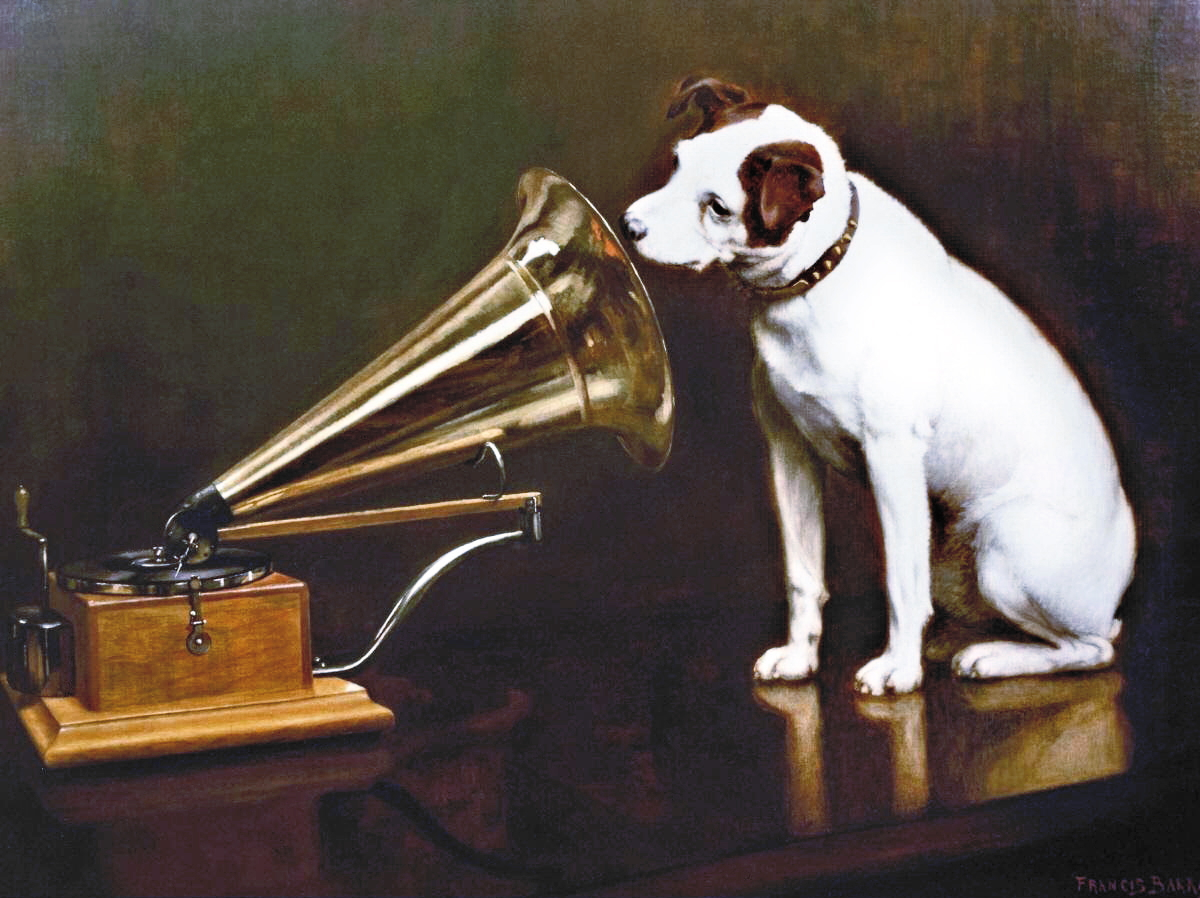
\includegraphics[width=2in]{Henry Thesis/Images/Original_Nipper}
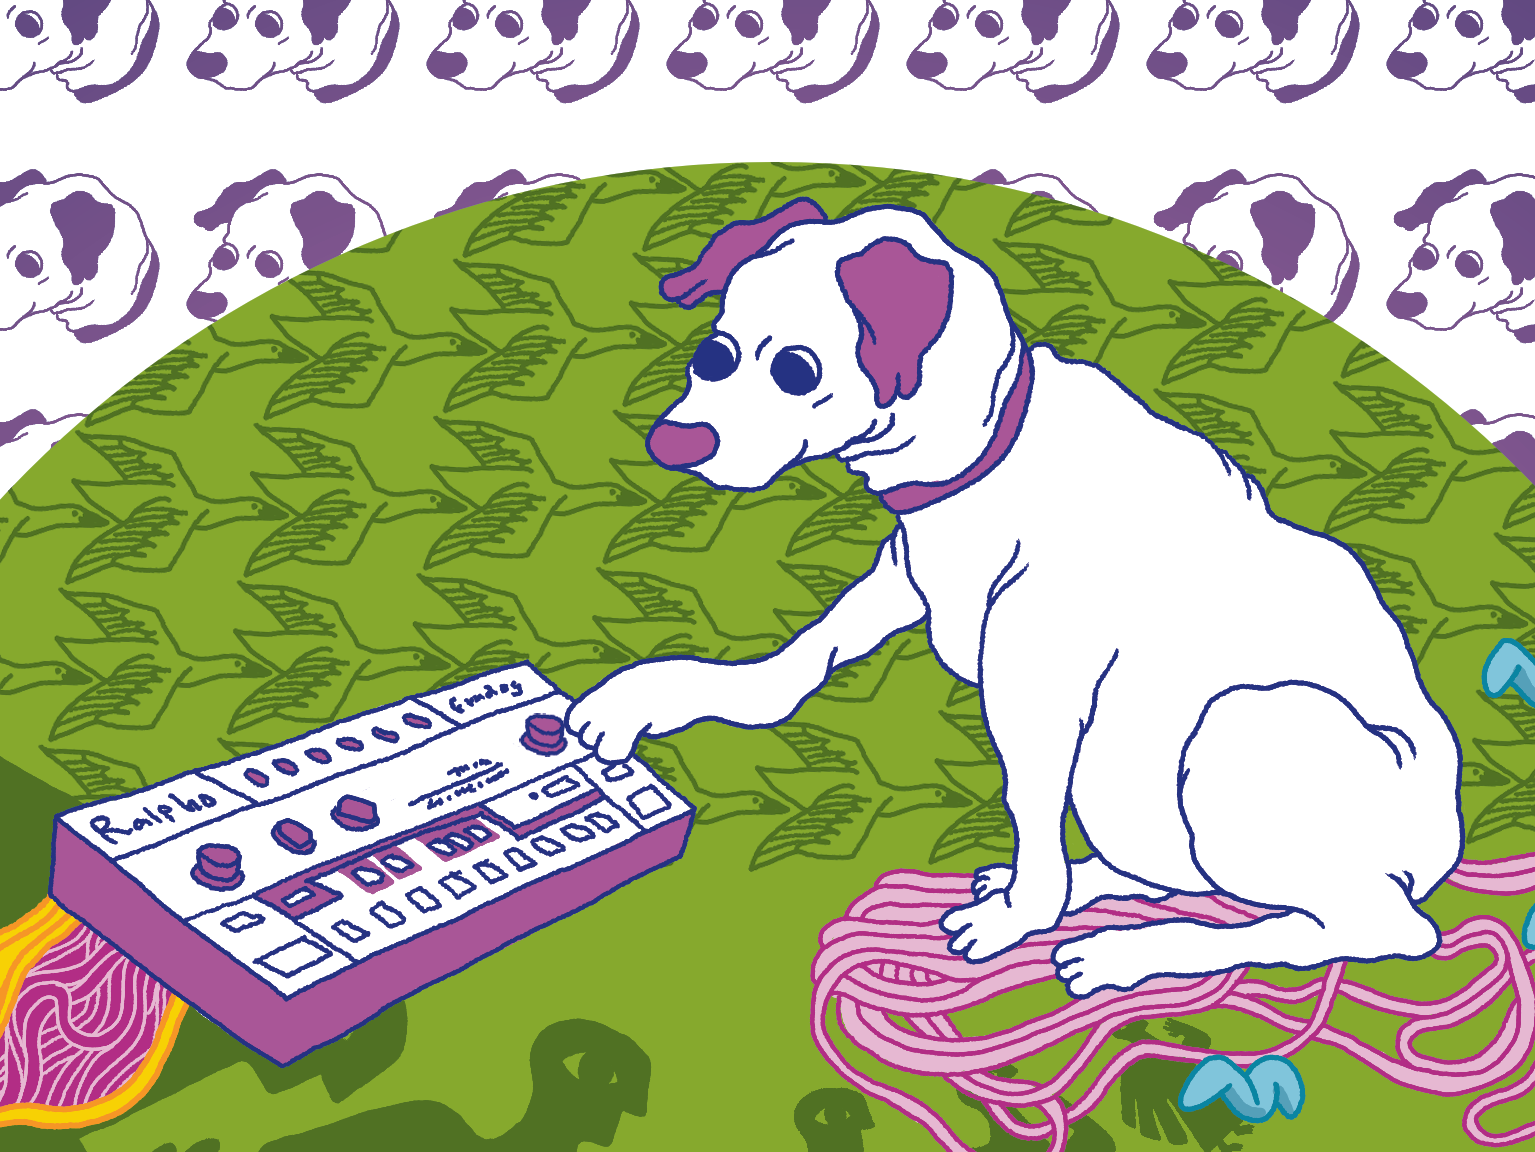
\includegraphics[width=2in]{Henry Thesis/Images/ALBUM_ART_DETAIL}
\caption{\emph{His Master's Voice} (c. 1898) by Francis Barraud, and a detail from \emph{Nipper Reigns Over a New Era of Consciousness} (2021) by Laurie Duffy}
\label{fig:dogcomparis}
\end{centering} 
\end{figure}


\section{Material Form}

I brought the final recordings to Murat {\c{C}}olak for mastering, a stage in the production process where a final polished version of the recording is made.\footnote{Information about Murat's engineering work is available at his website: \url{www.muratcolakmusic.com}} After a few mix adjustments on my end, Murat applied overall equalization, compression, saturation and limiting, among many other small refinements that created the final master. This resulted in a recording that translates better across listening platforms, and is ready to be made into a physical format.

To close the loop of inspiration from vinyl, I contracted the company Tangible Formats, which offers a service that can create limited runs of records.\footnote{Information about Tangible Formats is available here: \url{www.tangibleformats.com}} Instead of pressing vinyl out of molten plastic, each record is cut on a lathe in a blank vinyl disc. These records are similar to an acetate master disc which is the first step in the process of creating stampers to press records.\footnote{\cite{hooseTurningTablesEngineering2018}, 11-17.} Acetate masters discs have a history in dance music as a way to play the newest music, which could also be unfinished, or would never be fully released. These special discs are referred to as ``dubplates'' a term that comes from the origins of the practice in Jamaican sound system culture.\footnote{\cite{bennettDubplateCultureAnalogue}} In contrast to an acetate, which can wear out after 5 plays, the lifespan of a PVC record almost matches that of a pressed record.\footnote{Despite the name, ``acetate'' records contain no acetate, and are made from aluminum coated with a nitrocellulose lacquer.} I ordered several records to be cut by Tangible Formats, one of which is set to be stored in the Reed library. This means if you are reading my thesis in the year 2051, 2081, or 20021 and .wav and .mp3 files accompanying my thesis have gone missing or are now unplayable, chances are that the record remains. The final digital files will be accessible on the Reed Electronic Theses Archive.\footnote{The archive can be found, as of April 2021, at: \url{https://rdc.reed.edu/c/etheses/home/}}

\section{Conclusion}

Despite the discussion I have given minimalism, it remains a vague and open-ended term. Much of this is due to how the term can bend to fit different situations. Minimalism can mean sparsity and reduction, but even the densest pieces of musical composition can be minimalist at the core of their conception. Some minimalist works can be transparent in form, like the work of Robert Hood, Steve Reich and Sol LeWitt, or they can be made murky and obtuse, as with Basic Channel's generous use of delay and reverb which creates a texture all its own.

At the center of the term ``minimal'' I struck upon a practice of using small artistic gestures that are expanded through repetition and gradual modification to create a larger piece. A single musical idea interacts with itself through time to create something more complex, like a cube changes its impact on an observer when arranged with copies of itself.\footnote{\cite{lewittSeries123471968}} When small changes play out over time, the effect on the listener is pronounced. This creates expectations of change as Jeff Mills observed, and these expectations can either be satisfied or subverted.\footnote{\cite{schmidtJeffMillsLecture1998a}} In cases where a pattern breaks, it can startle the listener on these ideas, or through physical space, they can create far larger permutations. In other forms this might manifest as a rounding error repeated many times over, or a pattern that suddenly breaks and startles the observer.

My own interpretation of minimalism is also different from many of the artists I have discussed. The sculptors and musicians in the 1960s and 70s stated that they did not see their work as ``minimal'' and shunned the term when it was applied to their work. Others, like Jeff Mills and Robert Hood, embraced the term and approached it as an intentional aesthetic, adapting the meaning of ``minimal'' to fit their creative vision.

I did not see myself as a minimalist while composing either. I had to forget I was creating ``minimal'' artwork, otherwise I thought too much about whether my music was ``minimal enough.'' Instead, I focused on creating a small musical phrase and developing it. This meant I could write music and let the idea to grow larger without stopping to fret over perfection. Only in retrospect did I realize I managed to fit into the definition of minimalism I was working towards. I find myself now understanding minimalism as a creative process, rather than a specific aesthetic. The occasional austere aesthetics of minimalism, like clean digital percussion in techno and raw industrial materials in visual art, were not as important as I had first thought them to be. The common minimalist aesthetic choices are useful to make the effects of repetition more noticeable by removing confusing textures and patterns. At its most fundamental level, minimalism is a technique for repeating small forms, and using the repetition as a path for evolution, expression, and momentum.

%If you feel it necessary to include an appendix, it goes here.
\appendix

\chapter{Equipment}

For those interested, I have compiled a list of the tools I used through this project to lend further insight into my own creative process.
\subsection{Recording}
\begin{description}
    \item [ASUS Intel i7 Laptop (2017)]
    \item [Ableton Live 10 Suite] digital audio workstation
    \item [MOTU 828mk3] audio interface
    \item [Mackie 1604vl4] mixer
    \item [Adam T7v] studio monitors
    \item [Senneheiser HD-650] headphones
\end{description}
\subsection{Synthesizers and Samplers}
\begin{description}
    \item [Akai MPC2000xl] sampler and sequencer
    \item [Elektron Octatrack MKII] sampler and sequencer
    \item[Korg Minilogue] polyphonic analog synthesizer
    \item[Korg Monologue] monophonic analog synthesizer
    \item[Cyclone Analogic TT-303] Roland TB-303 clone, monophonic analog synthesizer
    \item[Roland TR8-S] drum machine and drum synthesizer, TR-909 emulator
\end{description}
\subsection{Effects}
\begin{description}
    \item[Strymong Volante] digital tape delay emulation pedal
    \item[Alesis Quadraverb] programmable multi-effect
    \item[Alesis Midiverb II] preprogrammed effect unit
\end{description}

%This is where endnotes are supposed to go, if you have them.
%I have no idea how endnotes work with LaTeX.

  \backmatter % backmatter makes the index and bibliography appear properly in the t.o.c...

% if you're using bibtex, the next line forces every entry in the bibtex file to be included
% in your bibliography, regardless of whether or not you've cited it in the thesis.
% \nocite{*}

% Rename my bibliography to be called "Works Cited" and not "References" or ``Bibliography''
% \renewcommand{\bibname}{Works Cited}

%\bibliographystyle{bsts/ChicagoReedweb} % there are a variety of styles available; 
%\bibliographystyle{plainnat}
% replace ``plainnat'' with the style of choice. You can refer to files in the bsts or APA 
% subfolder, e.g. 
%\bibliographystyle{APA/apa-good}  % or
%\bibliography{thesis}
 % Comment the above two lines and uncomment the next line to use biblatex-chicago.

\printbibliography[heading=bibintoc,nottype=music,title={References}]
\printbibliography[heading=subbibintoc,type=music,title={Discography}]

% Finally, an index would go here... but it is also optional.
\end{document}
